
\begin{sidewaystable}
	\centering
	\caption{Pulsar timing data for 47\,Tuc, spin periods. Reference key is as follows:
		a:\citet{Freire2018}, b:\citet{Freire2017}, c:\citet{Ridolfi2016}}

	\begin{tabular}{c c c c c c c c}
		\hline

		ID\textsuperscript{reference} & $r$ [arcmin] & $P$ [ms]         & $\Delta P$ [ms] & $\dot{P}$ [s/s]     & $\Delta \dot{P}$ [s/s] & DM [pc/cm3] & $\Delta$DM [pc/cm3] \\
		\hline
		aa\textsuperscript{a}         & 0.465        & 1.8453805296800  & \num{6 E-13}    & \num{-4.5890E-20}   & \num{0.0015E-20}       & 24.971      & 0.007               \\
		ab\textsuperscript{b}         & 0.2092       & 3.7046394947985  & \num{5 E-13}    & \num{9.820E-21}     & \num{0.008E-21}        & 24.373      & 0.020               \\
		c\textsuperscript{b}          & 1.2298       & 5.7567799955164  & \num{1 E-13}    & \num{-49.850E-21}   & \num{0.002E-21}        & 24.600      & 0.004               \\
		D\textsuperscript{b}          & 0.6483       & 5.35757328486572 & \num{7E-14}     & \num{-3.4219E-21}   & \num{0.0009E-21}       & 24.732      & 0.003               \\
		E\textsuperscript{b}          & 0.6205       & 3.53632915276243 & \num{3E-14}     & \num{98.5103E-21}   & \num{0.0005E-21}       & 24.236      & 0.004               \\
		F\textsuperscript{b}          & 0.2149       & 2.62357935251262 & \num{3E-14}     & \num{64.5031E-21}   & \num{0.0007E-21}       & 24.382      & 0.005               \\
		G\textsuperscript{b}          & 0.2781       & 4.0403791435651  & \num{1 E-13}    & \num{-42.159E-21}   & \num{0.002E-21}        & 24.436      & 0.004               \\
		H\textsuperscript{b}          & 0.7677       & 3.2103407093504  & \num{1 E-13}    & \num{-1.830E-21}    & \num{0.001E-21}        & 24.369      & 0.008               \\
		I\textsuperscript{b}          & 0.2772       & 3.4849920616629  & \num{1 E-13}    & \num{-45.873E-21}   & \num{0.002E-21}        & 24.429      & 0.010               \\
		J\textsuperscript{b}          & 1.0185       & 2.10063354535248 & \num{6E-14}     & \num{-9.7919E-21}   & \num{0.0009E-21}       & 24.588      & 0.003               \\
		L\textsuperscript{b}          & 0.1627       & 4.3461679994616  & \num{3 E-13}    & \num{-122.0406E-21} & \num{0.0010E-21}       & 24.400      & 0.012               \\
		M\textsuperscript{b}          & 1.0688       & 3.6766432176002  & \num{3 E-13}    & \num{-38.418E-21}   & \num{0.005E-21}        & 24.432      & 0.016               \\
		N\textsuperscript{b}          & 0.4793       & 3.0539543462608  & \num{1 E-13}    & \num{-21.857E-21}   & \num{0.002E-21}        & 24.574      & 0.009               \\
		O\textsuperscript{b}          & 0.0806       & 2.64334329724356 & \num{4E-14}     & \num{30.3493E-21}   & \num{0.0006E-21}       & 24.356      & 0.002               \\
		Q\textsuperscript{b}          & 0.9502       & 4.0331811845726  & \num{2 E-13}    & \num{34.0076E-21}   & \num{0.0006E-21}       & 24.265      & 0.004               \\
		R\textsuperscript{b}          & 0.1519       & 3.4804627074933  & \num{2 E-13}    & \num{148.351E-21}   & \num{0.003E-21}        & 24.361      & 0.007               \\
		S\textsuperscript{b}          & 0.2150       & 2.83040595787912 & \num{7E-14}     & \num{-120.541E-21}  & \num{0.001E-21}        & 24.376      & 0.004               \\
		T\textsuperscript{b}          & 0.3179       & 7.5884798073671  & \num{9 E-13}    & \num{293.80E-21}    & \num{0.01E-21}         & 24.411      & 0.021               \\
		U\textsuperscript{b}          & 0.9386       & 4.3428266963923  & \num{1 E-13}    & \num{95.228E-21}    & \num{0.002E-21}        & 24.337      & 0.004               \\
		W\textsuperscript{c}          & 0.087        & 2.3523445319370  & \num{3 E-13}    & \num{-8.6553E-20}   & \num{0.0001E-20}       & 24.367      & 0.003               \\
		X\textsuperscript{c}          & 3.828        & 4.77152291069355 & \num{5E-14}     & \num{1.83609E-20}   & \num{0.00007E-20}      & 24.539      & 0.005               \\
		Y\textsuperscript{b}          & 0.3743       & 2.19665714352124 & \num{6E-14}     & \num{-35.1720E-21}  & \num{0.0008E-21}       & 24.468      & 0.004               \\
		Z\textsuperscript{b}          & 0.1506       & 4.554447383906   & \num{3  E-12}   & \num{-4.56E-21}     & \num{0.1E-21}          & 24.450      & 0.040               \\
		\hline
	\end{tabular}

	\label{tab:pulsars_spin}

\end{sidewaystable}


\begin{sidewaystable}
	\centering
	\caption{Pulsar timing data for 47\,Tuc, orbital periods. Reference key is as follows:
		a:\citet{Freire2018}, b:\citet{Freire2017}, c:\citet{Ridolfi2016}}

	\begin{tabular}{c c c c c c c c}
		\hline

		ID\textsuperscript{reference} & $r$ [arcmin] & $P_b$ [day]   & $\Delta P_b$ [day] & $\dot{P_b}$ [s/s] & $\Delta \dot{P_b}$ [s/s] & DM [pc/cm3] & $\Delta$DM [pc/cm3] \\

		\hline
		E\textsuperscript{b}          & 0.6205       & 2.2568483     & 0.0000009          & \num{4.8E-12}     & \num{0.2E-12}            & 24.236      & 0.004               \\
		H\textsuperscript{b}          & 0.7677       & 2.357696895   & 0.000000010        & \num{-0.7E-12}    & \num{0.6E-12}            & 24.369      & 0.008               \\
		I\textsuperscript{b}          & 0.2772       & 0.2297922489  & 0.0000000004       & \num{-0.8E-12}    & \num{0.2E-12}            & 24.429      & 0.010               \\
		Q\textsuperscript{b}          & 0.9502       & 1.1890840496  & 0.0000000004       & \num{-1.0E-12}    & \num{0.2E-12}            & 24.265      & 0.004               \\
		R\textsuperscript{b}          & 0.1519       & 0.06623147751 & 0.00000000006      & \num{0.19E-12}    & \num{0.04E-12}           & 24.361      & 0.007               \\
		S\textsuperscript{b}          & 0.2150       & 1.2017242354  & 0.0000000006       & \num{-4.9E-12}    & \num{0.4E-12}            & 24.376      & 0.004               \\
		T\textsuperscript{b}          & 0.3179       & 1.126176771   & 0.000000001        & \num{2.5E-12}     & \num{1.1E-12}            & 24.411      & 0.021               \\
		U\textsuperscript{b}          & 0.9386       & 0.42910568324 & 0.00000000008      & \num{0.66E-12}    & \num{0.05E-12}           & 24.337      & 0.004               \\
		X\textsuperscript{c}          & 3.828        & 10.921183545  & 0.000000001        & \num{6E-12}       & \num{2E-12}              & 24.539      & 0.005               \\
		Y\textsuperscript{b}          & 0.3743       & 0.5219386107  & 0.0000000001       & \num{-0.82E-12}   & \num{0.07E-12}           & 24.468      & 0.004               \\
		\hline
	\end{tabular}

	\label{tab:pulsars_orbital}

\end{sidewaystable}




\begin{figure}
	\centering
	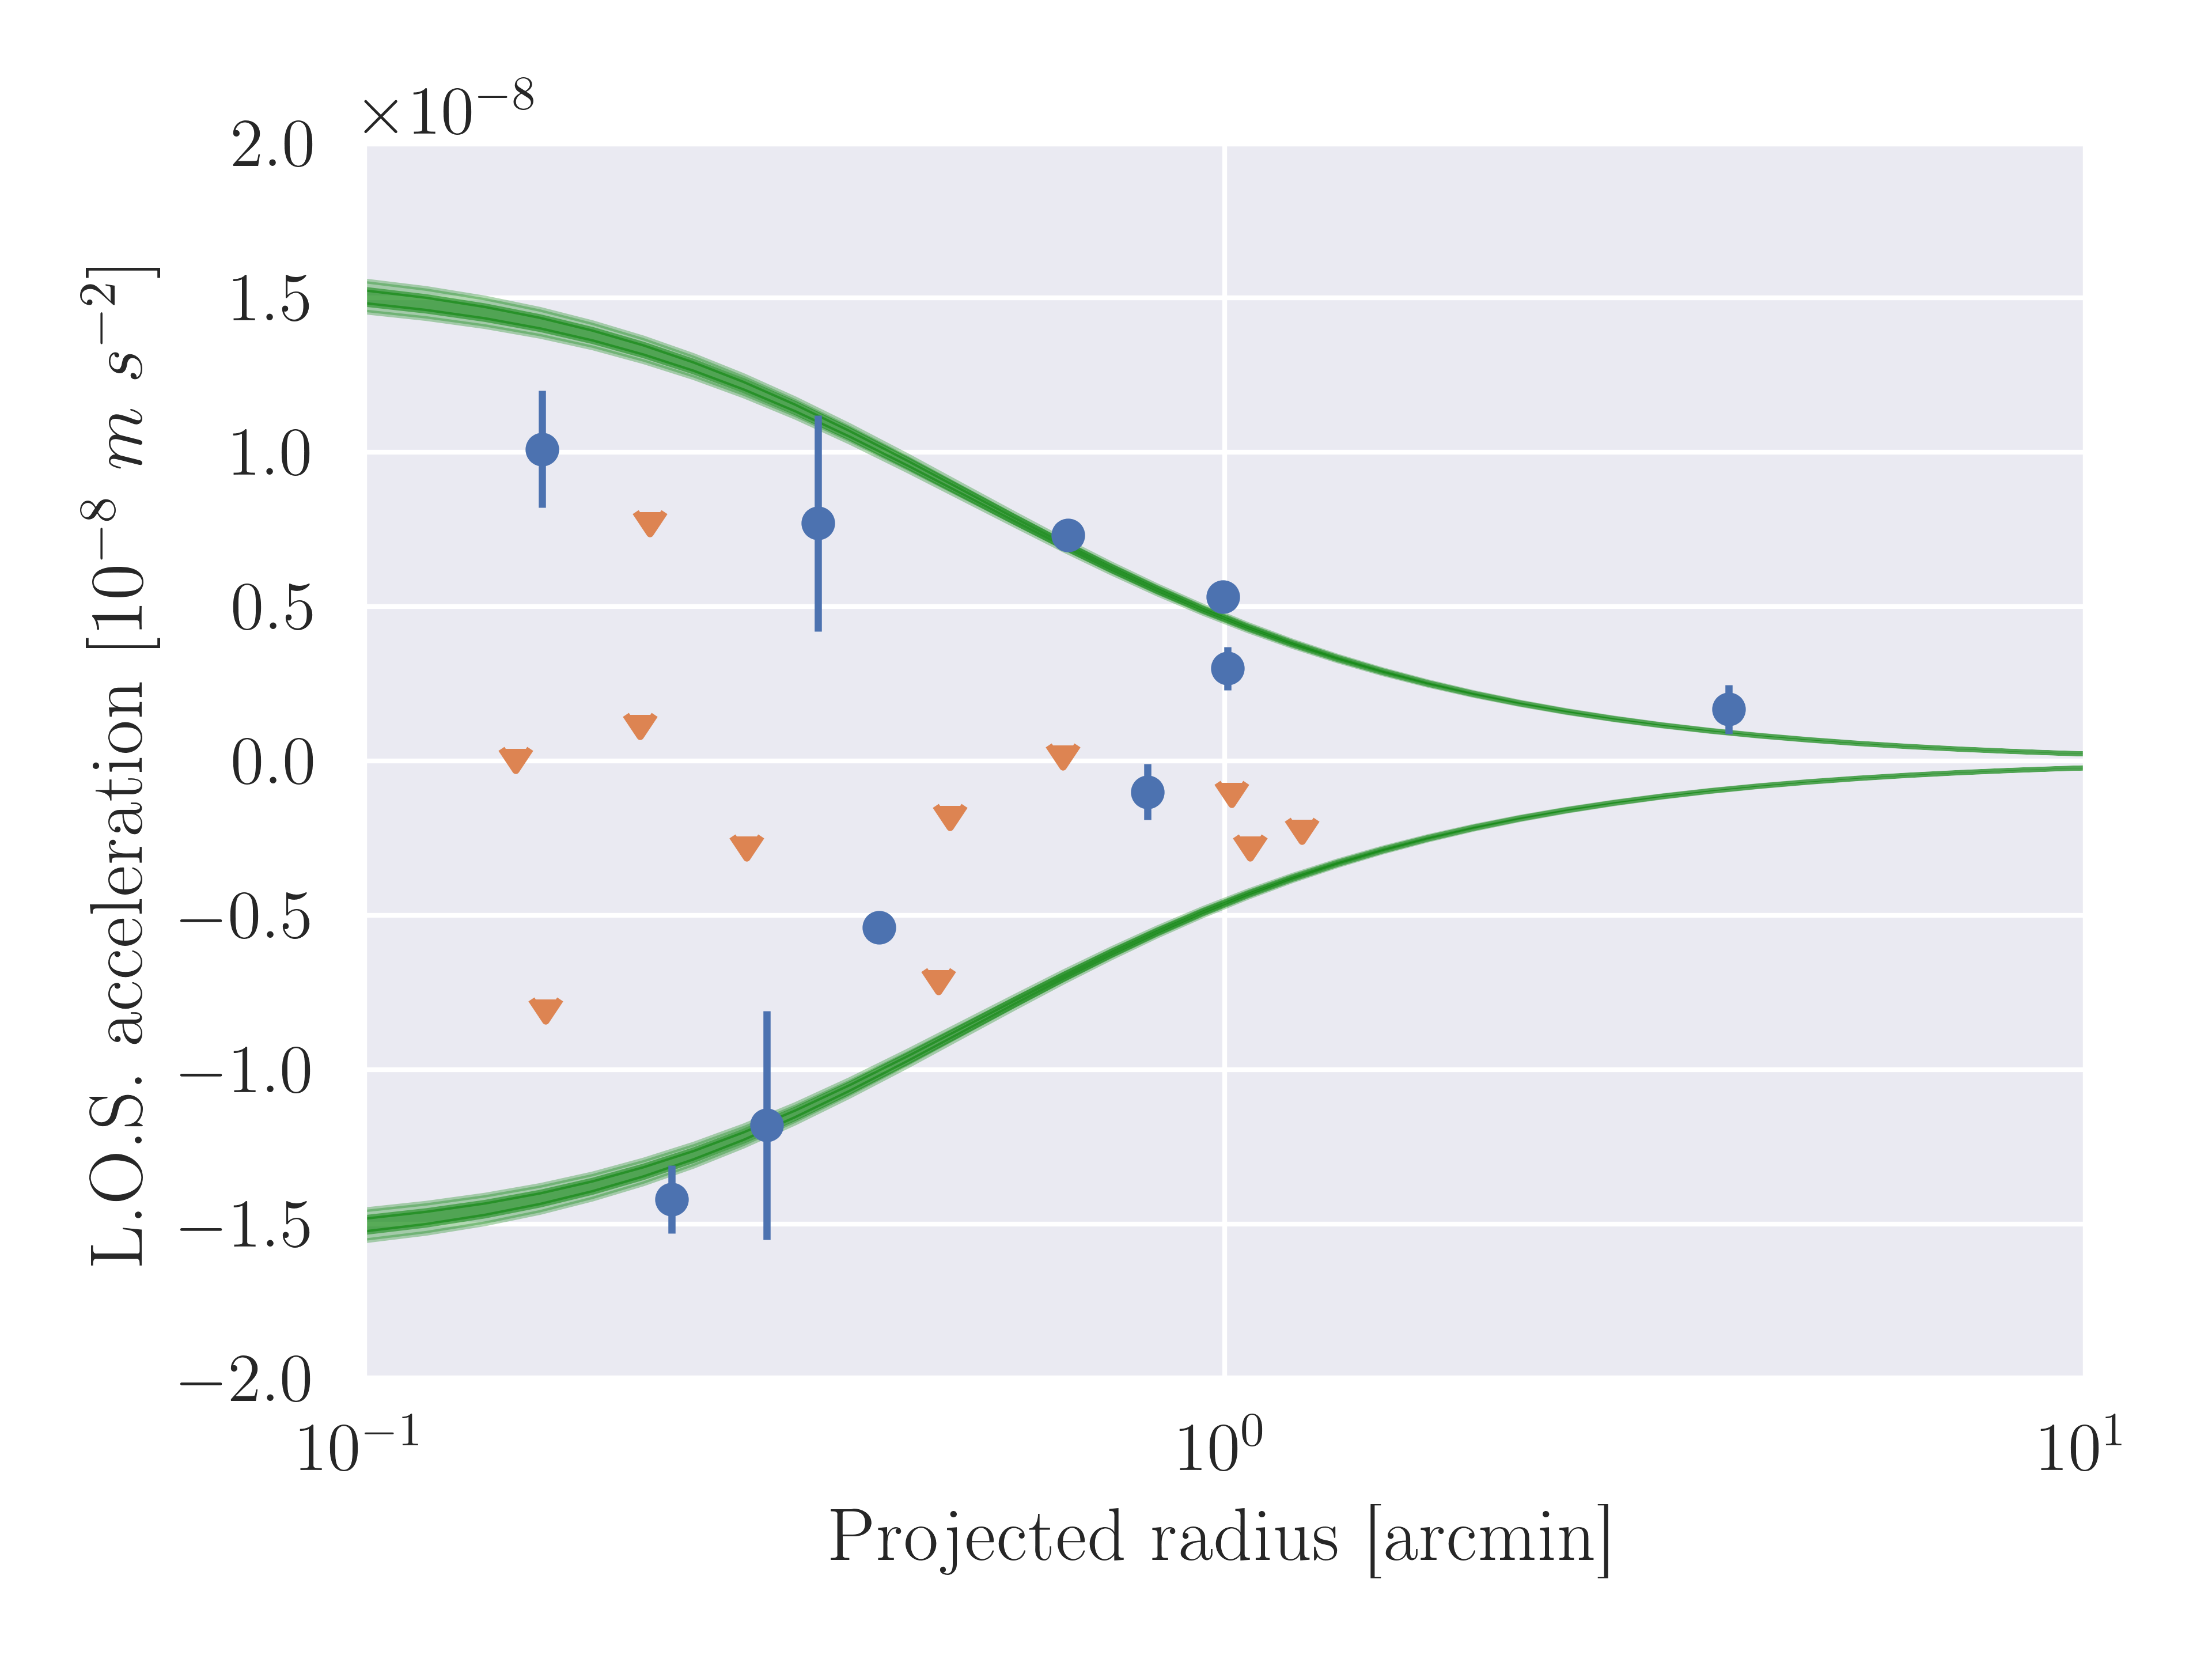
\includegraphics[width=0.9\textwidth]{figures/pulsar_posteriors/max_az_contours.png}
	\caption{Maximum acceleration profiles for set of best-fit models with a $0\%$ binary
		fraction. The accelerations of the pulsars, as derived from their period derivates,
		are plotted with accelerations derived from orbital periods in blue and upper limits
		for accelerations derived from spin periods in orange. All accelerations are
		consistent with the maximum acceleration allowed by the model within their 1
		$\sigma$ credibility intervals.}
	\label{fig:pulsar_max_az}
\end{figure}

\begin{figure}
	\centering
	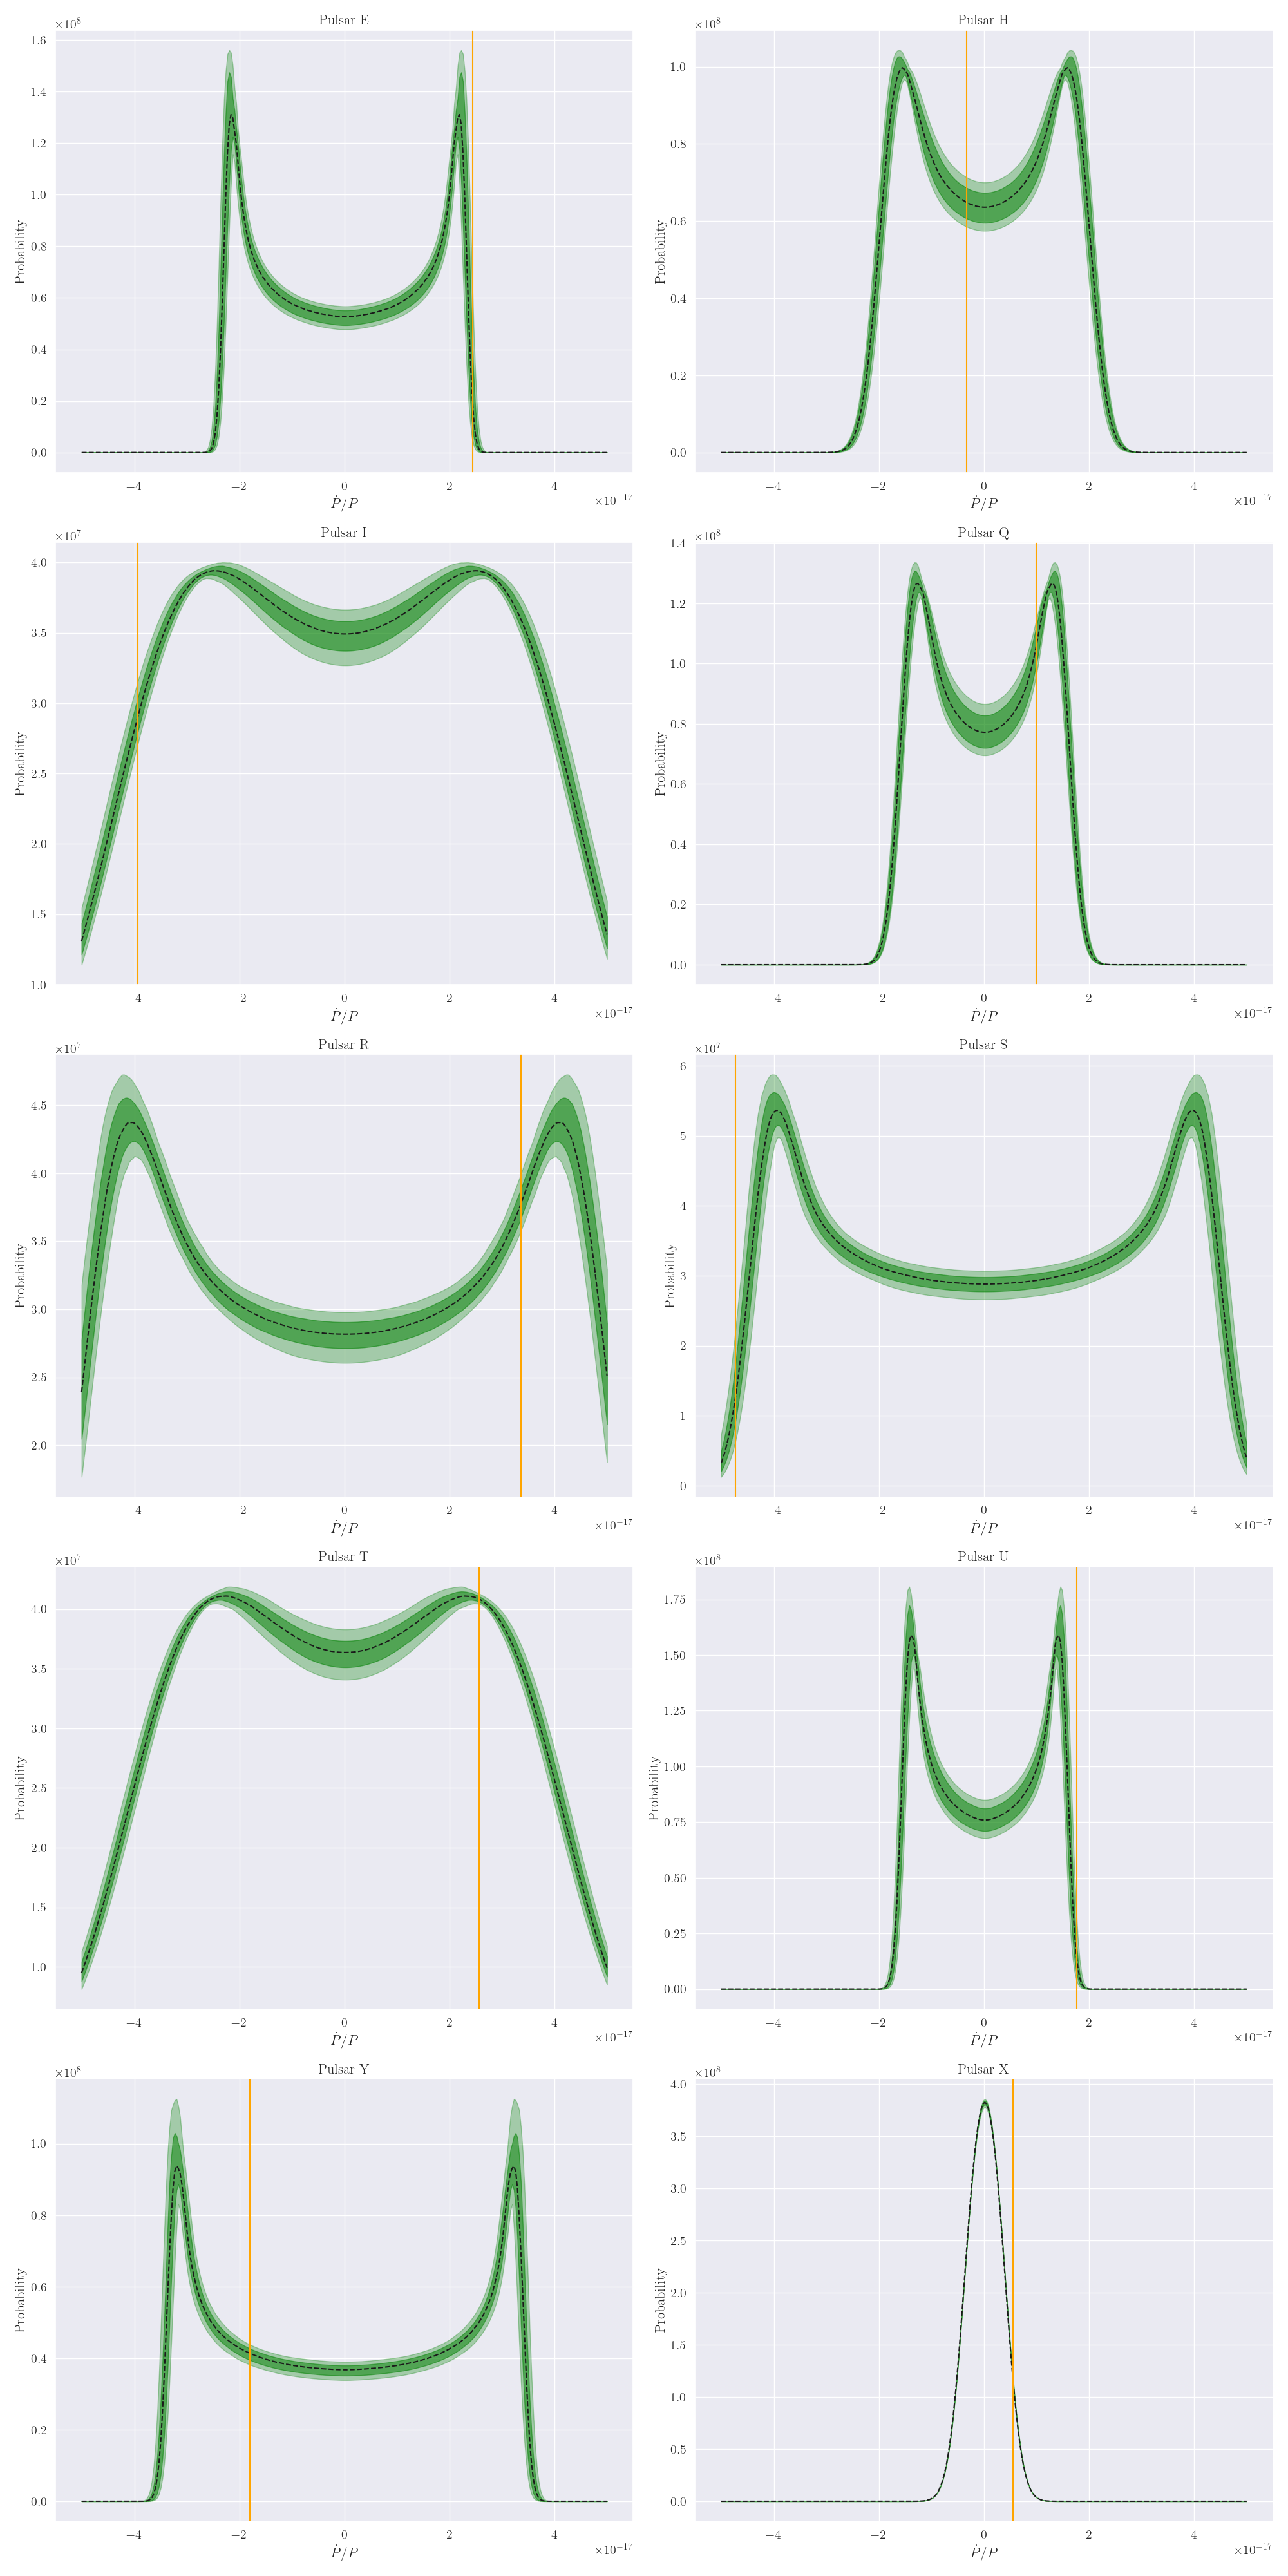
\includegraphics[width=0.7\textwidth]{figures/pulsar_posteriors/Paz.png}
	\caption{Probability distributions for measurements of orbital period derivatives for a set
		of best-fit models with a $0\%$ binary fraction. The measured period derivates for
		each pulsar are plotted in orange. }
	\label{fig:pulsar_Paz_orbital}
\end{figure}

\begin{sidewaysfigure}
	\centering
	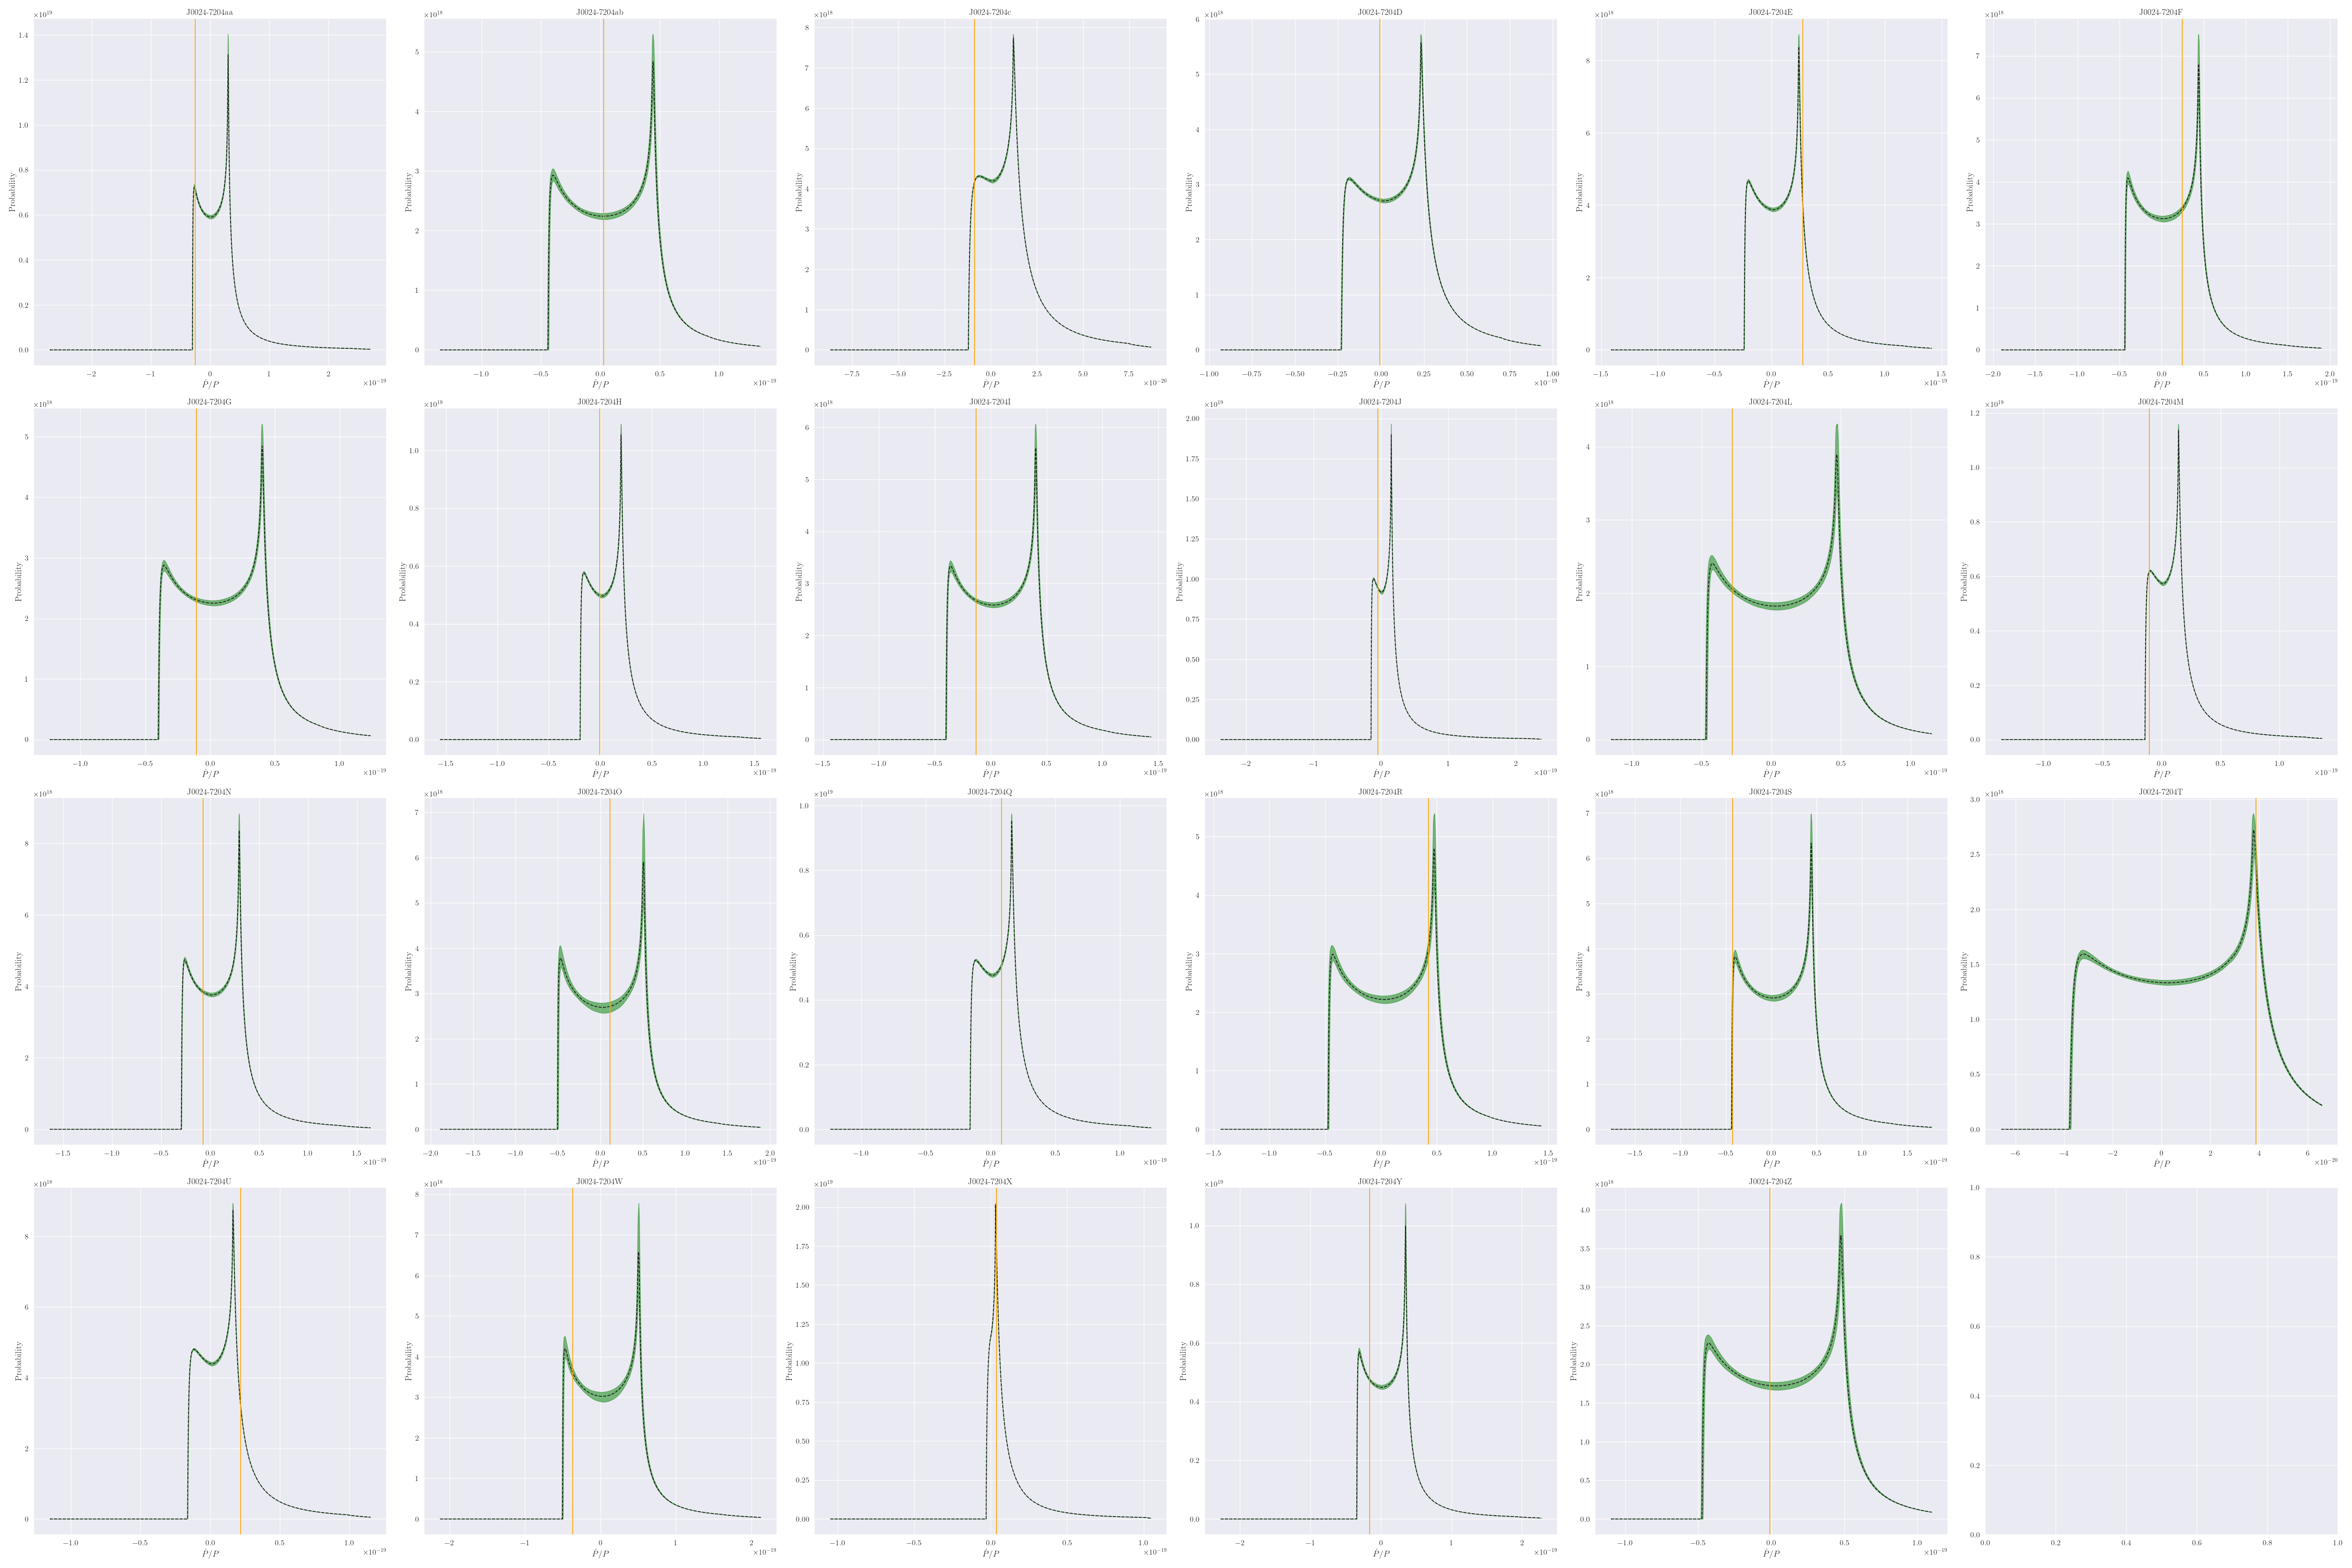
\includegraphics[width=0.9\textwidth]{figures/pulsar_posteriors/Paz_spin.png}
	\caption{Probability distributions for measurements of spin period derivatives for a set of
		best-fit models with a $0\%$ binary fraction. The measured period derivates for each
		pulsar are plotted in orange. }
	\label{fig:pulsar_Paz_spin}
\end{sidewaysfigure}



%%% Walker and Trace Plots

%%% Nobin
\begin{figure}
	\centering
	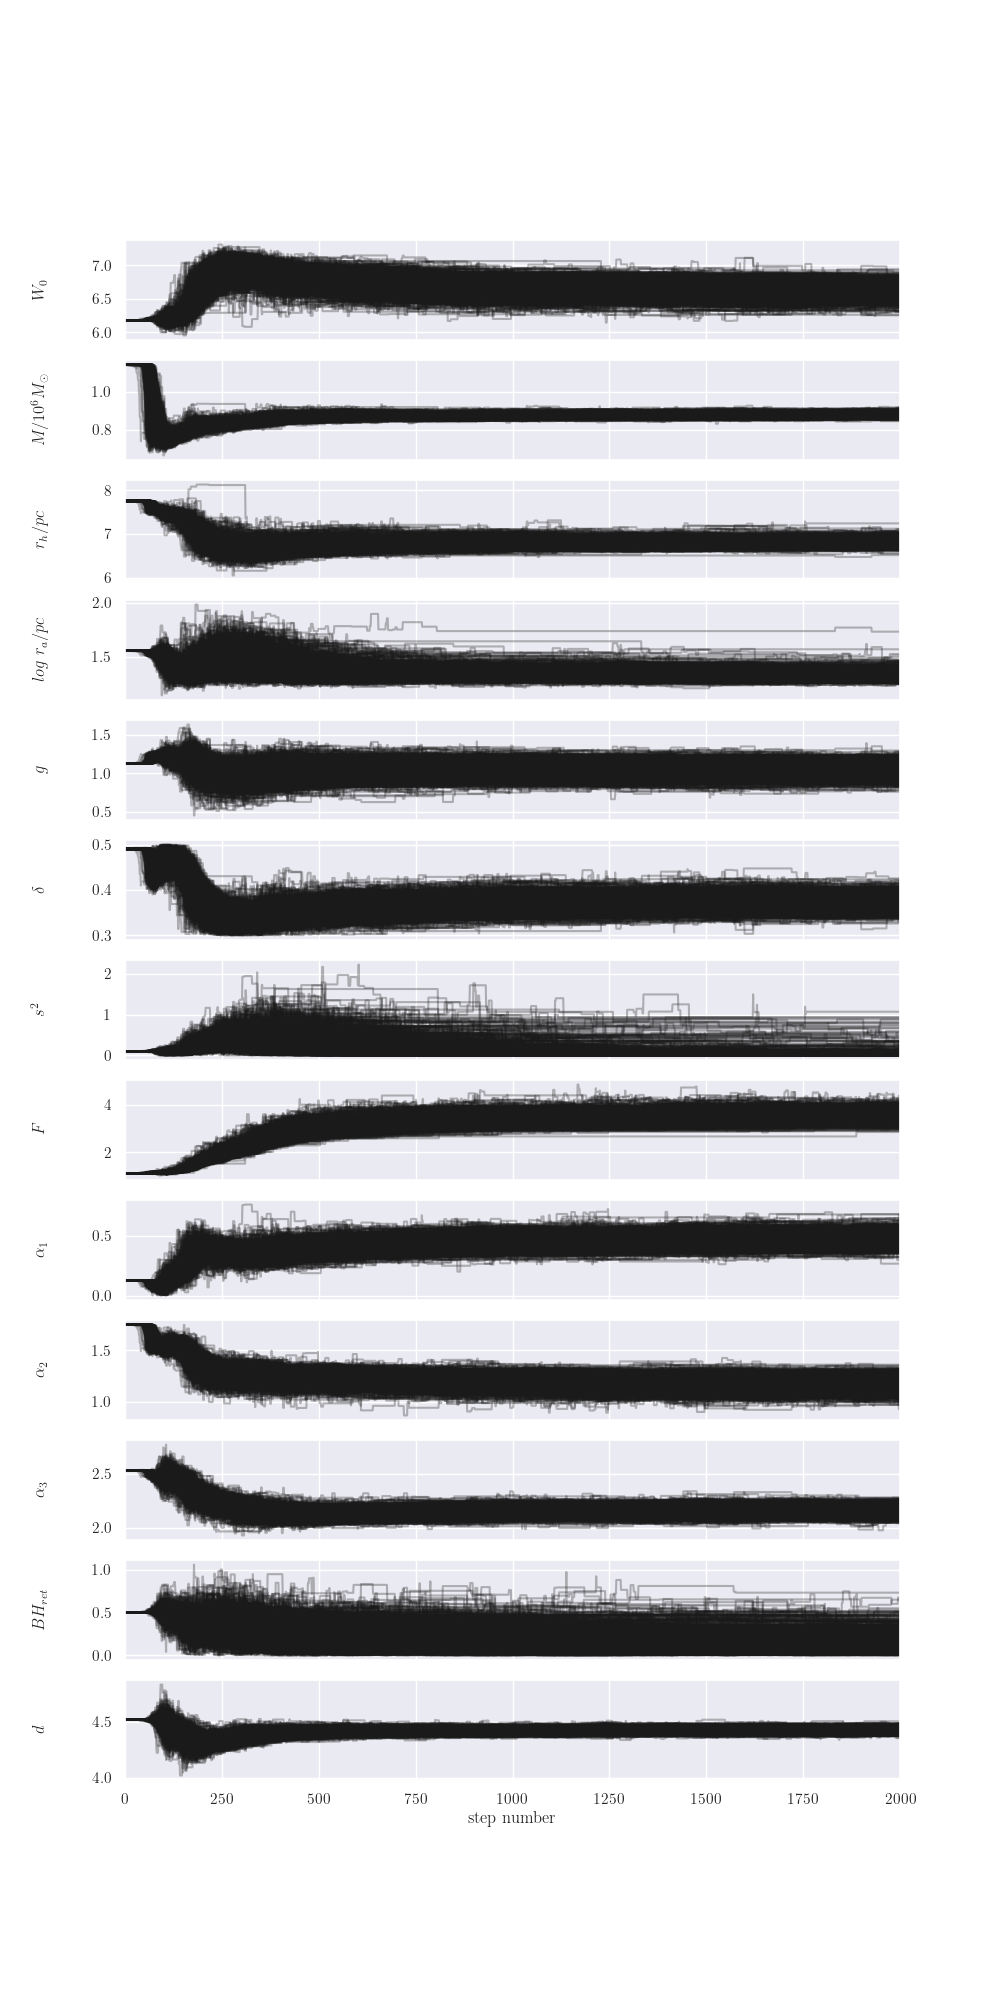
\includegraphics[width=0.7\textwidth]{figures/prev_nobin/walkers.png}
	\caption{Trace plot showing the evolution of the MCMC chain for model with a $0\%$ binary
		fraction.}
	\label{fig:nobin_walkers}
\end{figure}

\begin{figure}
	\centering
	\includegraphics[width=\textwidth]{figures/prev_nobin/corner.png}
	\caption{Corner plot showing the marginalized posterior probability distributions of models
		parameters with a $0\%$ binary fraction.}
	\label{fig:nobin_corner}
\end{figure}


%%% Lowbin
\begin{figure}
	\centering
	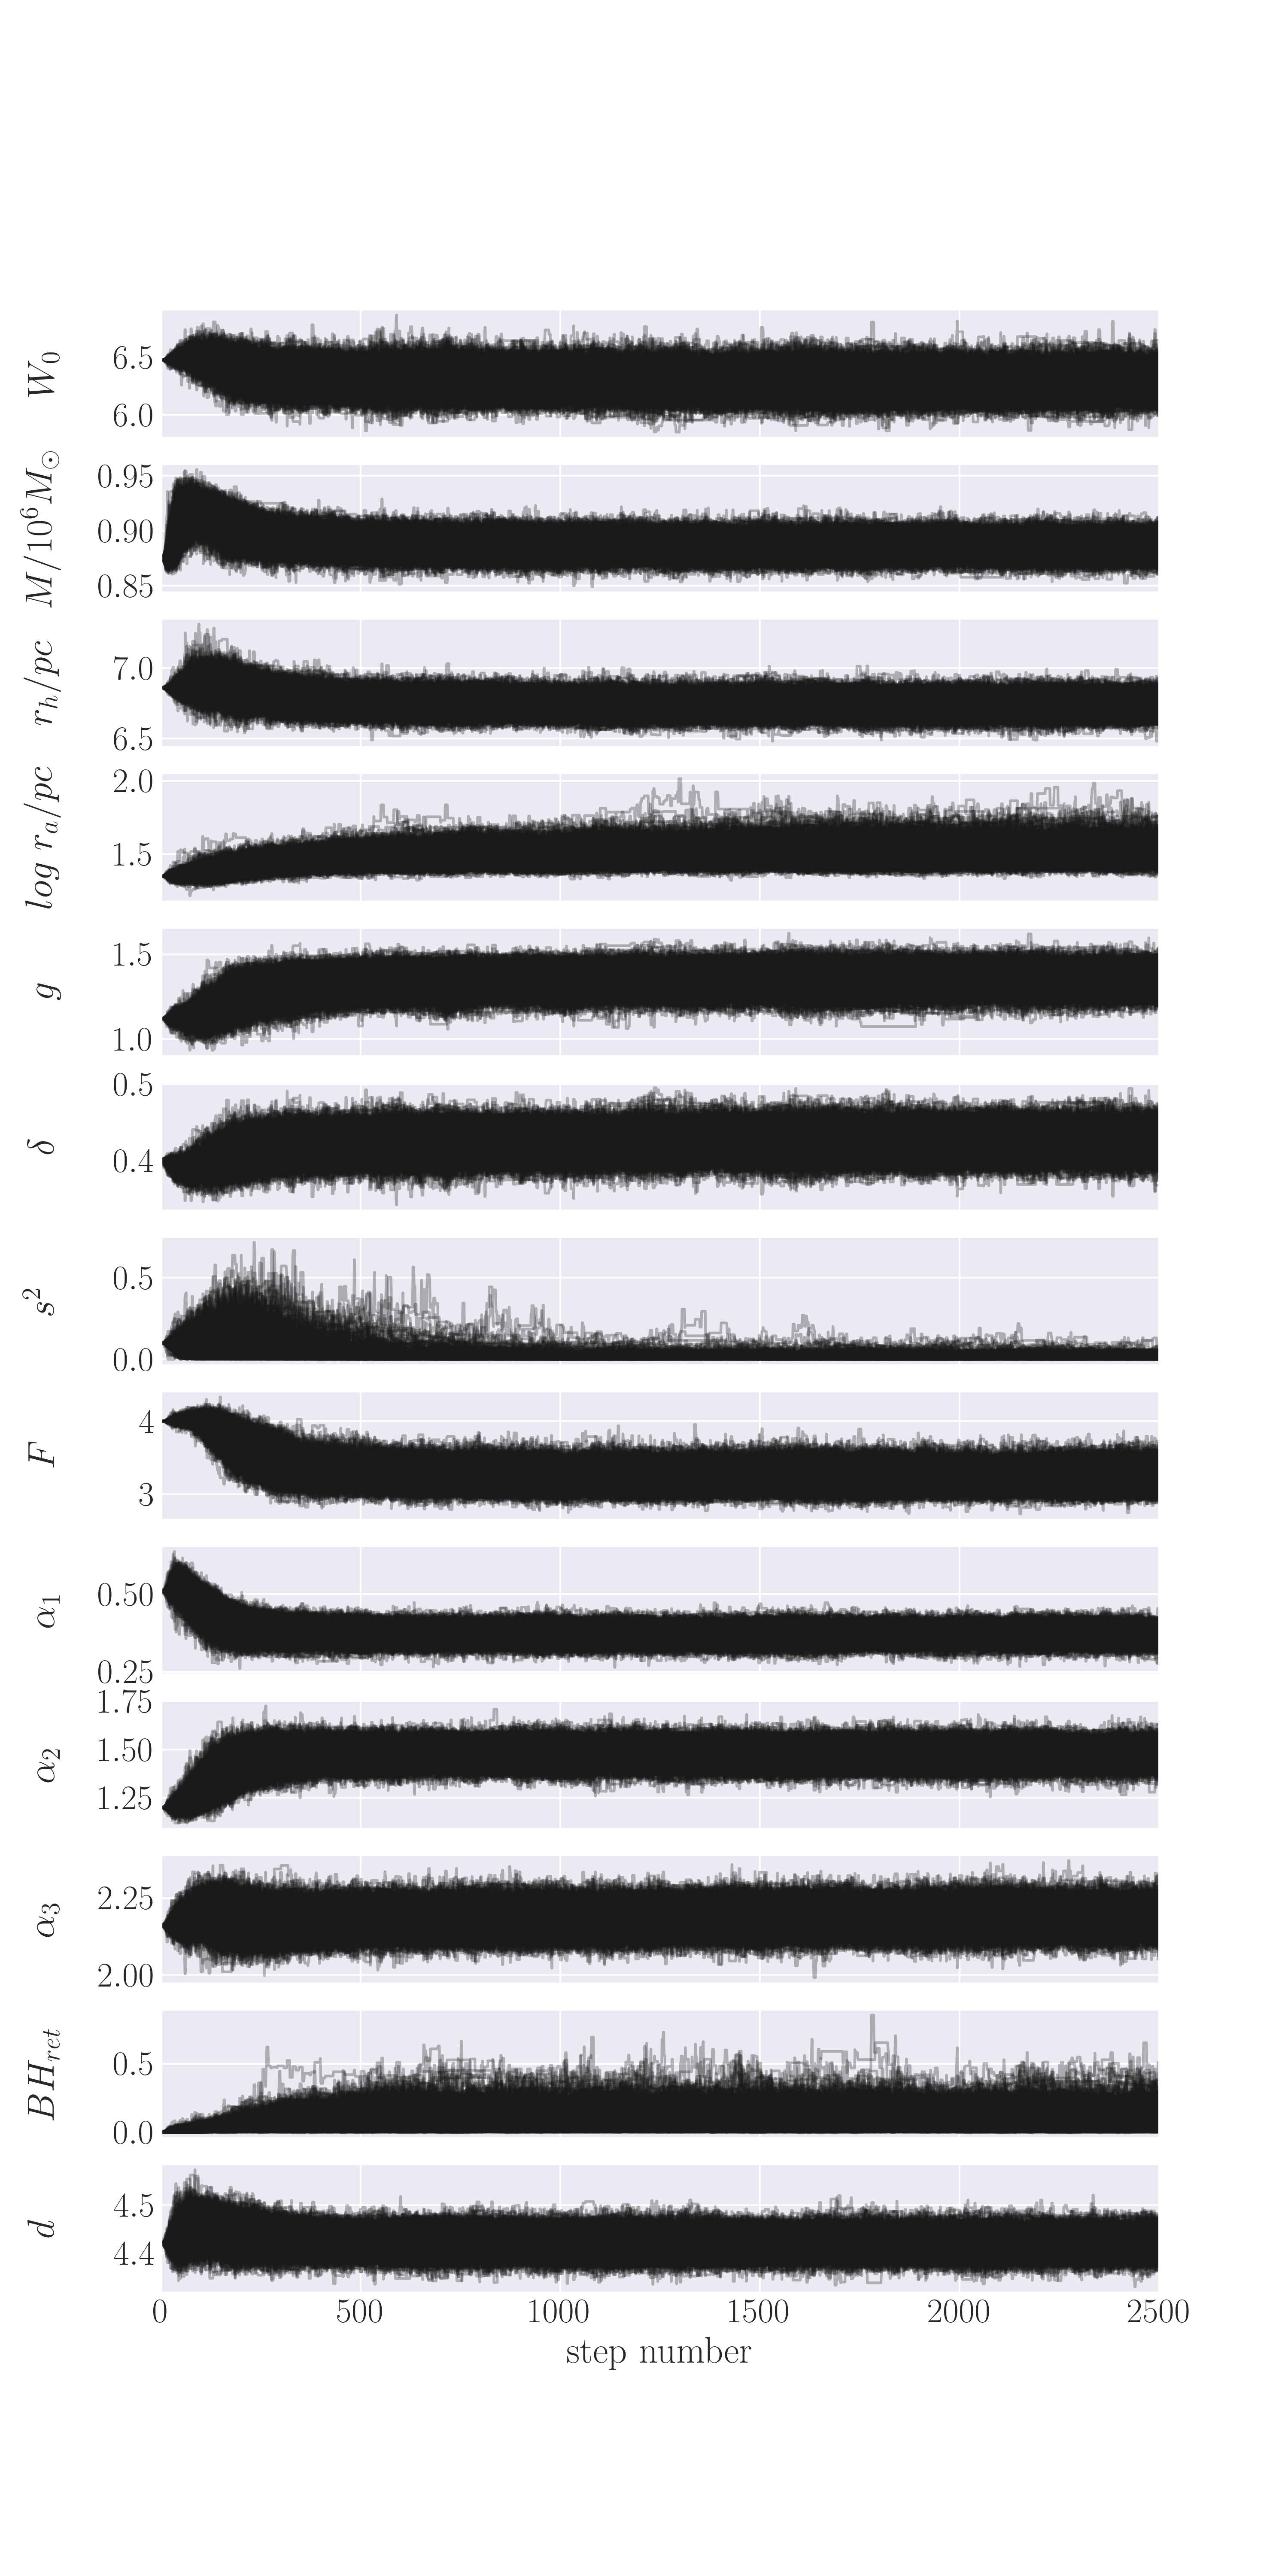
\includegraphics[width=0.7\textwidth]{figures/low_bin_model/walkers.png}
	\caption{Trace plot showing the evolution of the MCMC chain for model with a $2\%$ binary
		fraction.}
	\label{fig:lowbin_walkers}
\end{figure}

\begin{figure}
	\centering
	\includegraphics[width=\textwidth]{figures/low_bin_model/corner.png}
	\caption{Corner plot showing the marginalized posterior probability distributions of models
		parameters with a $2\%$ binary fraction.}
	\label{fig:lowbin_corner}
\end{figure}



%%% Highbin
\begin{figure}
	\centering
	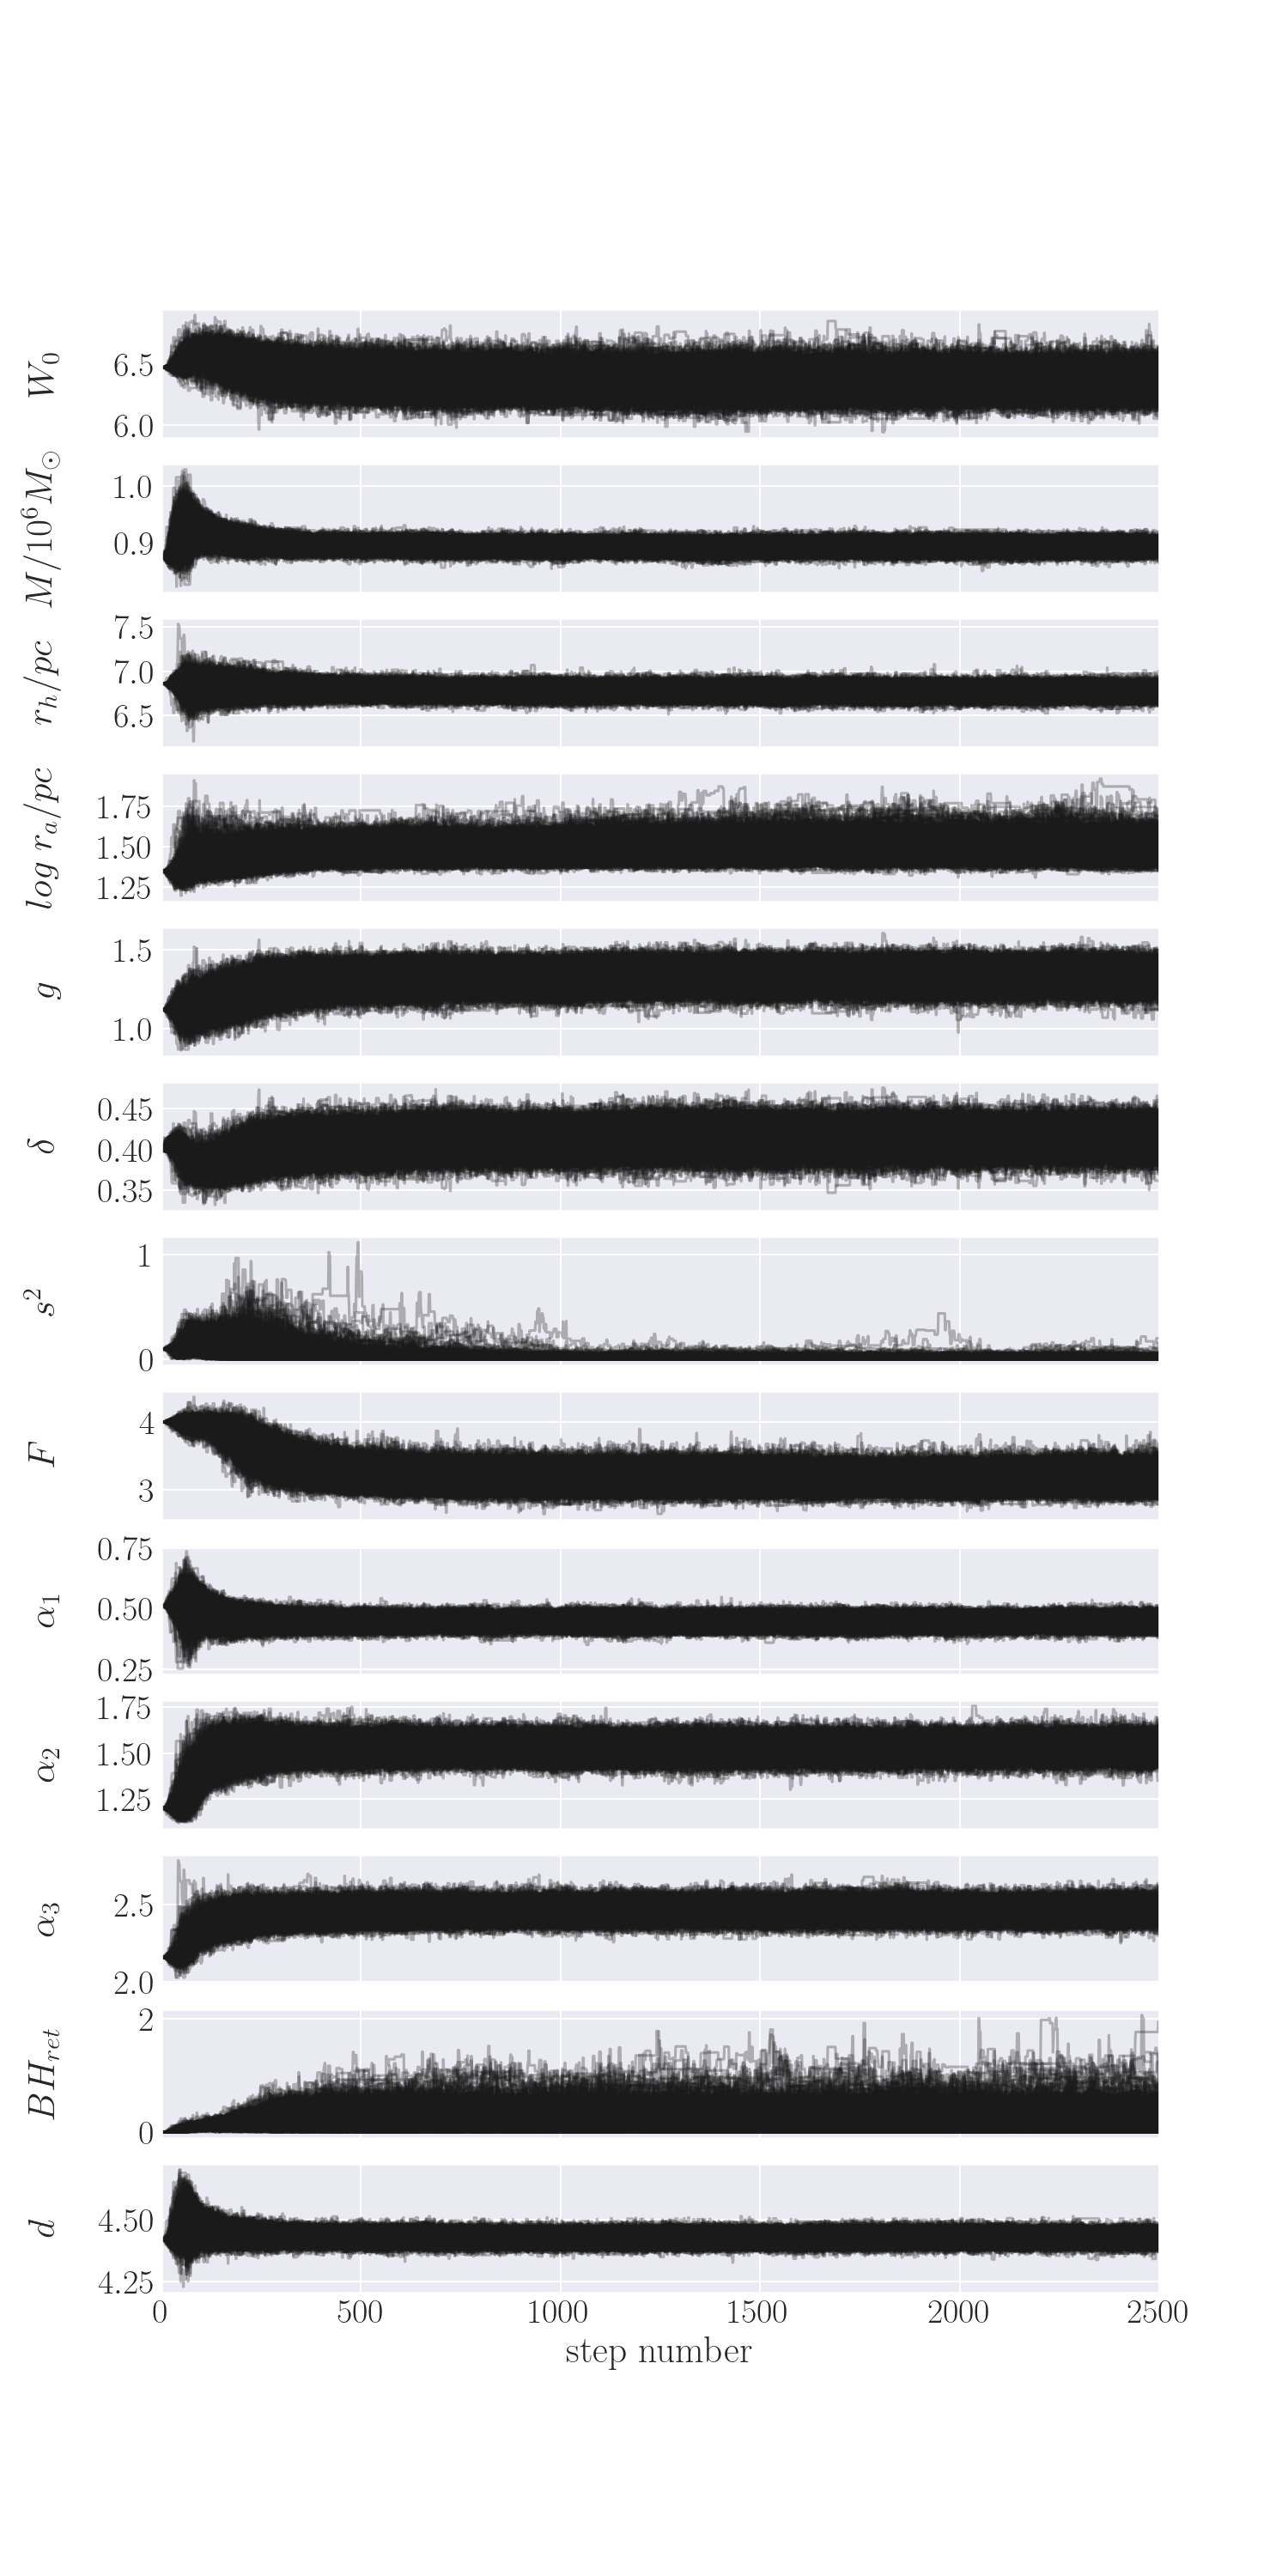
\includegraphics[width=0.7\textwidth]{figures/high_bin_model/walkers.png}
	\caption{Trace plot showing the evolution of the MCMC chain for model with a $10\%$ binary
		fraction.}
	\label{fig:highbin_walkers}
\end{figure}

\begin{figure}
	\centering
	\includegraphics[width=\textwidth]{figures/high_bin_model/corner.png}
	\caption{Corner plot showing the marginalized posterior probability distributions of models
		parameters with a $10\%$ binary fraction.}
	\label{fig:highbin_corner}
\end{figure}




%%% More Obs plots


%%% Nobin
\begin{figure}
	\begin{center}
		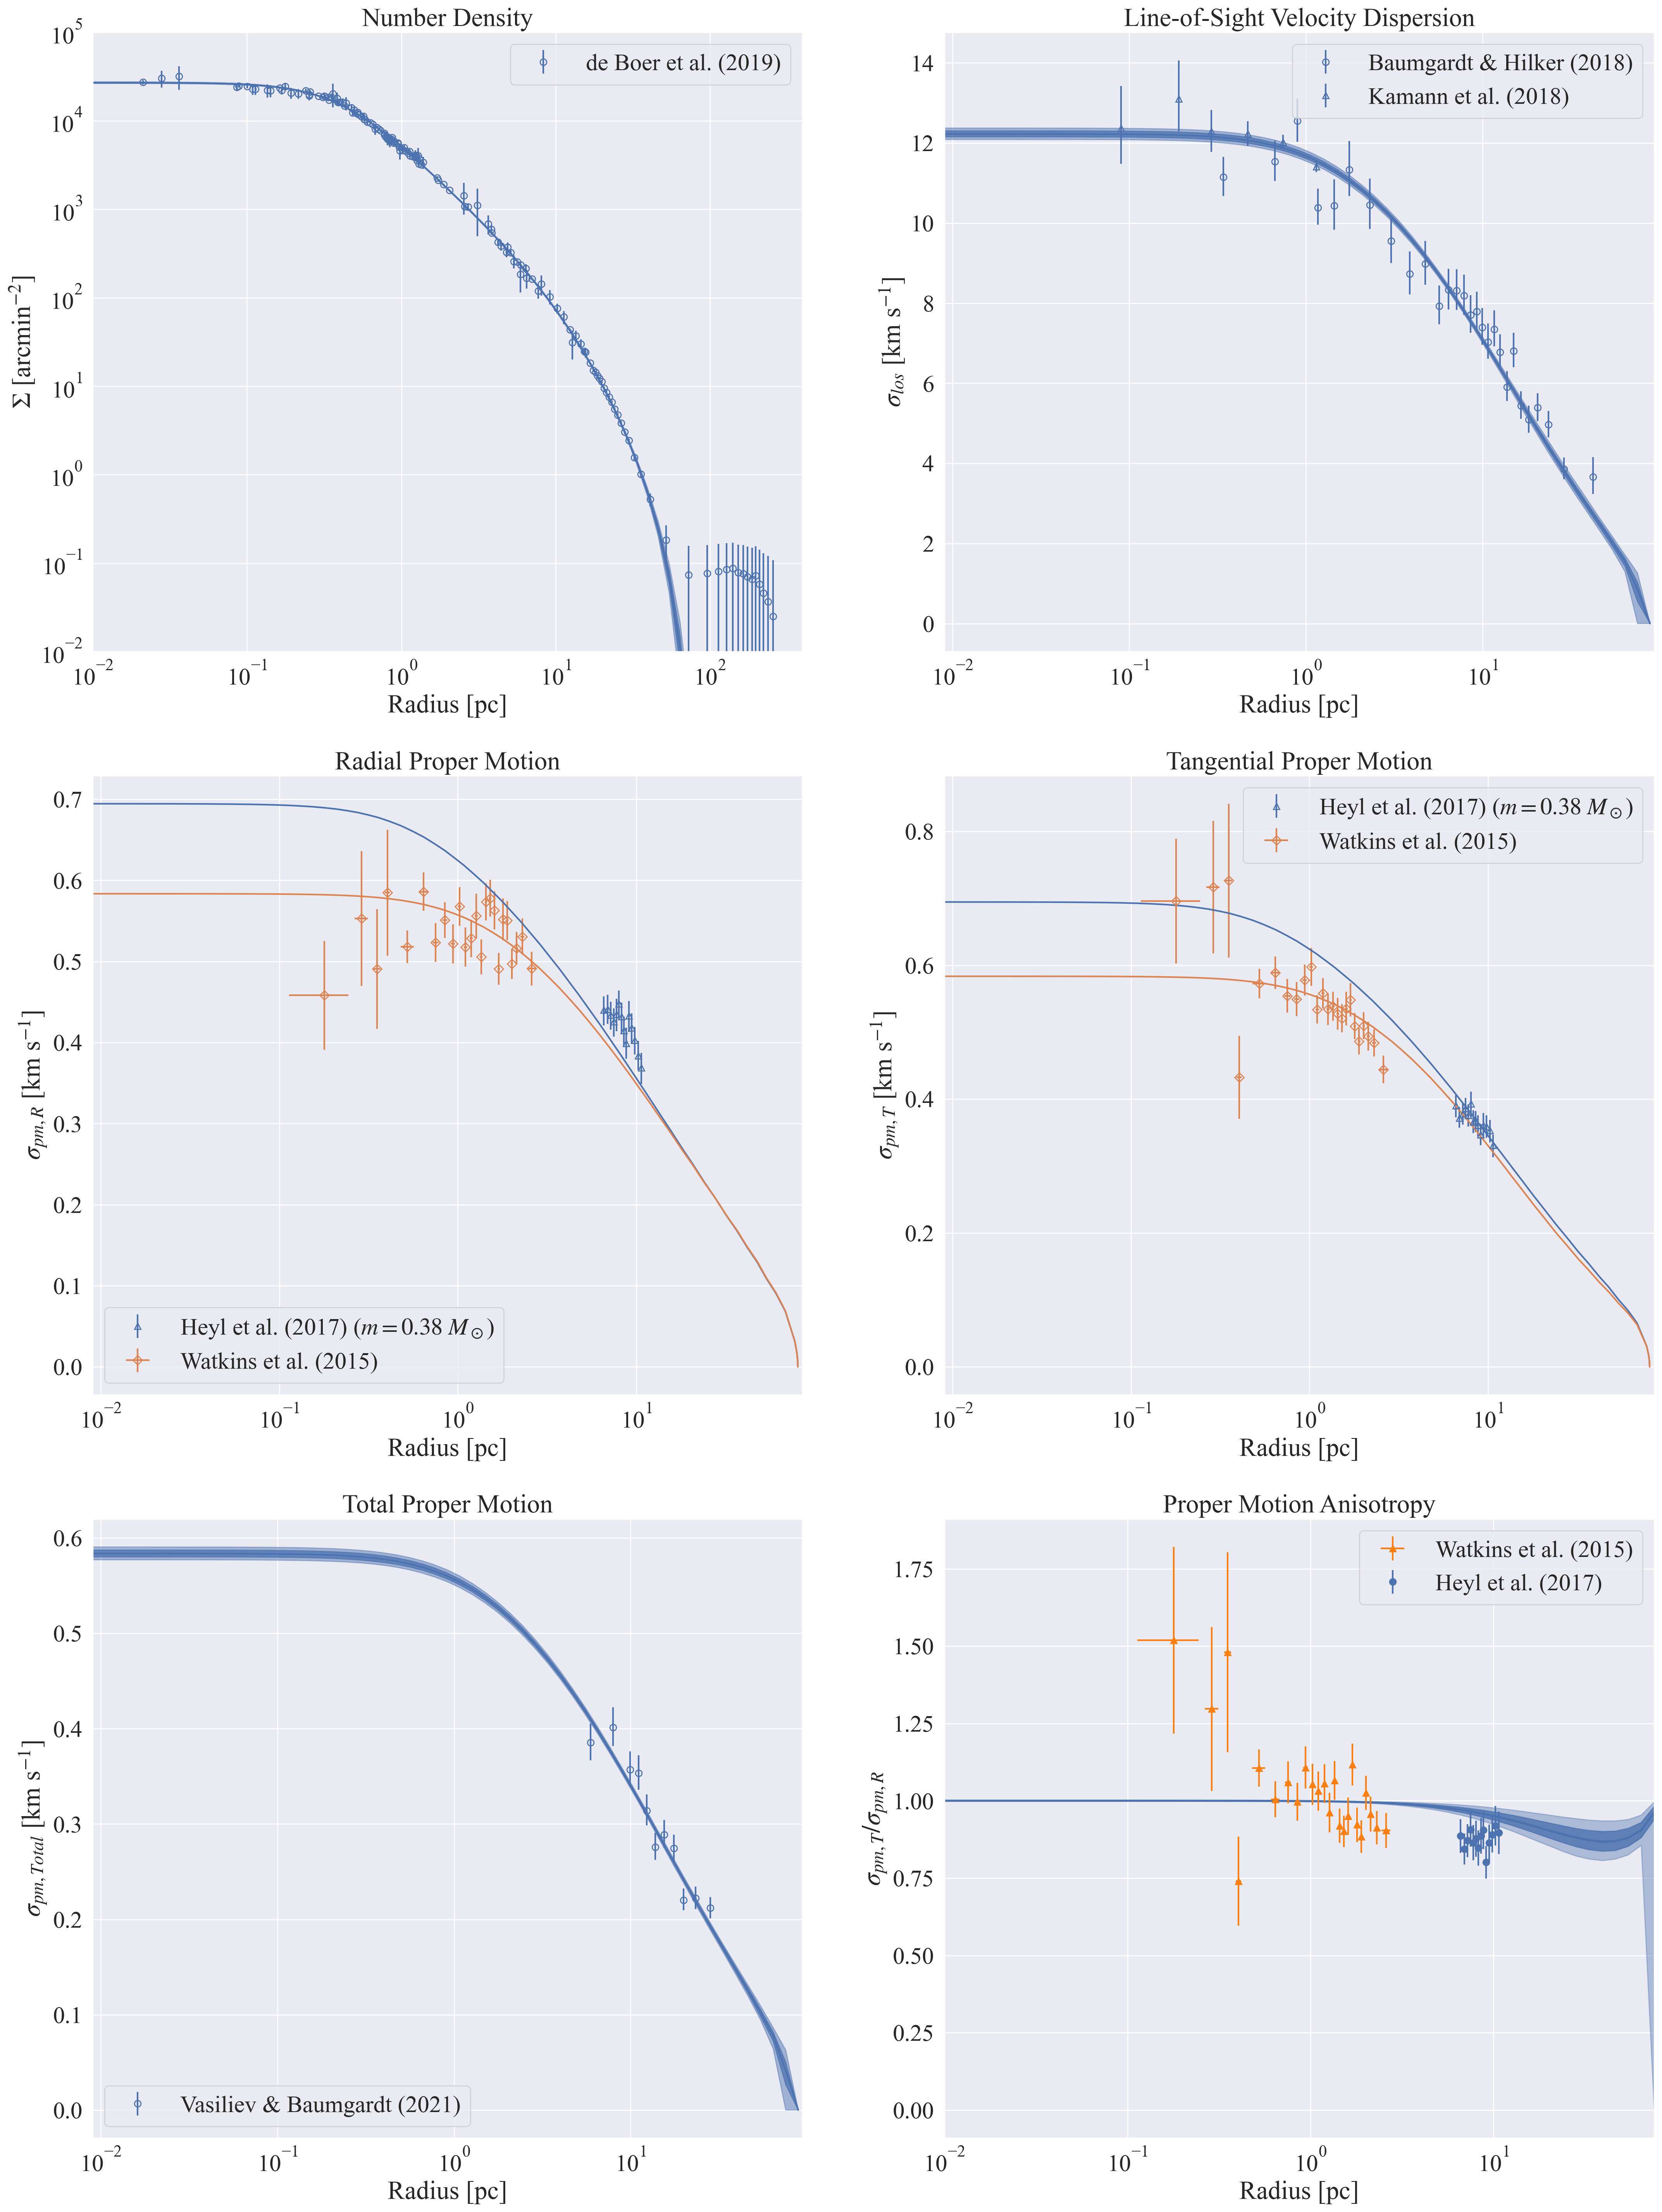
\includegraphics[width=0.9\textwidth]{figures/prev_nobin/obs_panel.png}
	\end{center}
	\caption{Model fits to the observables for models with no binary stars.}
	\label{fig:nobin_obs_panel}
\end{figure}

\begin{figure}
	\begin{center}
		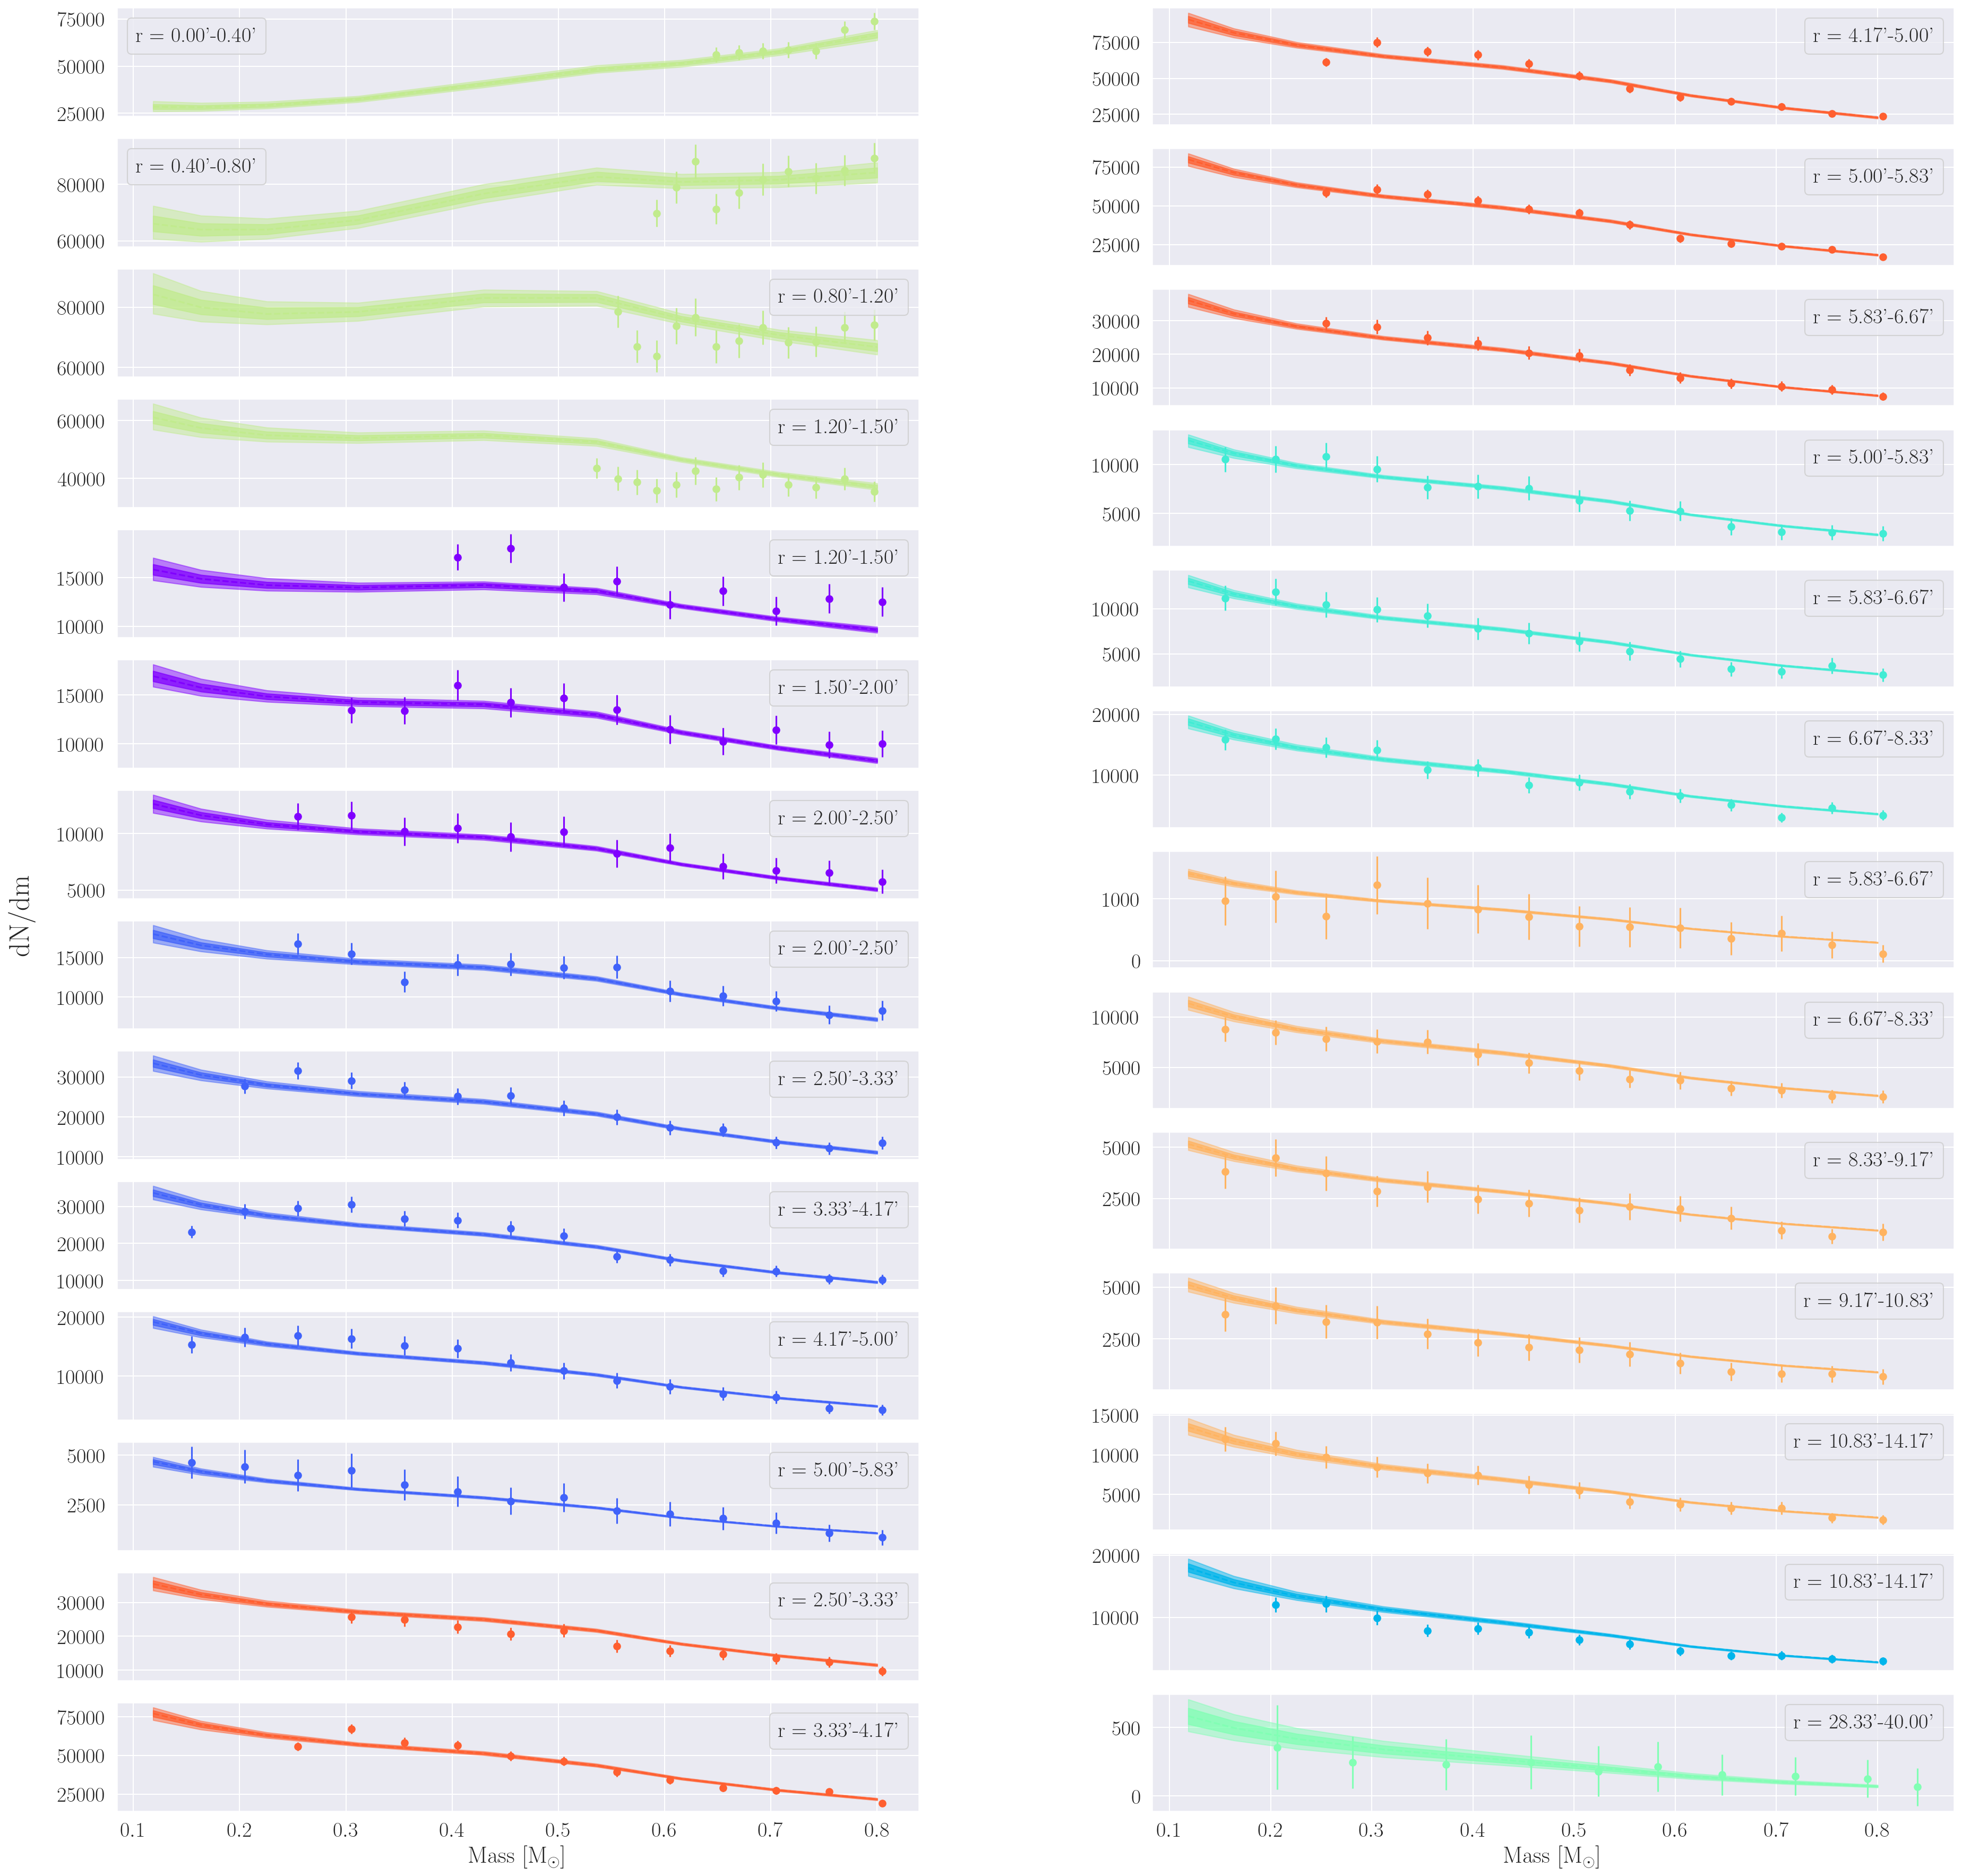
\includegraphics[width=0.9\textwidth]{figures/prev_nobin/mass_fun.png}
	\end{center}
	\caption{Model fits to stellar mass function data for models with no binary stars.}
	\label{fig:nobin_mass_fun}
\end{figure}


%%% Highbin
\begin{figure}
	\centering
	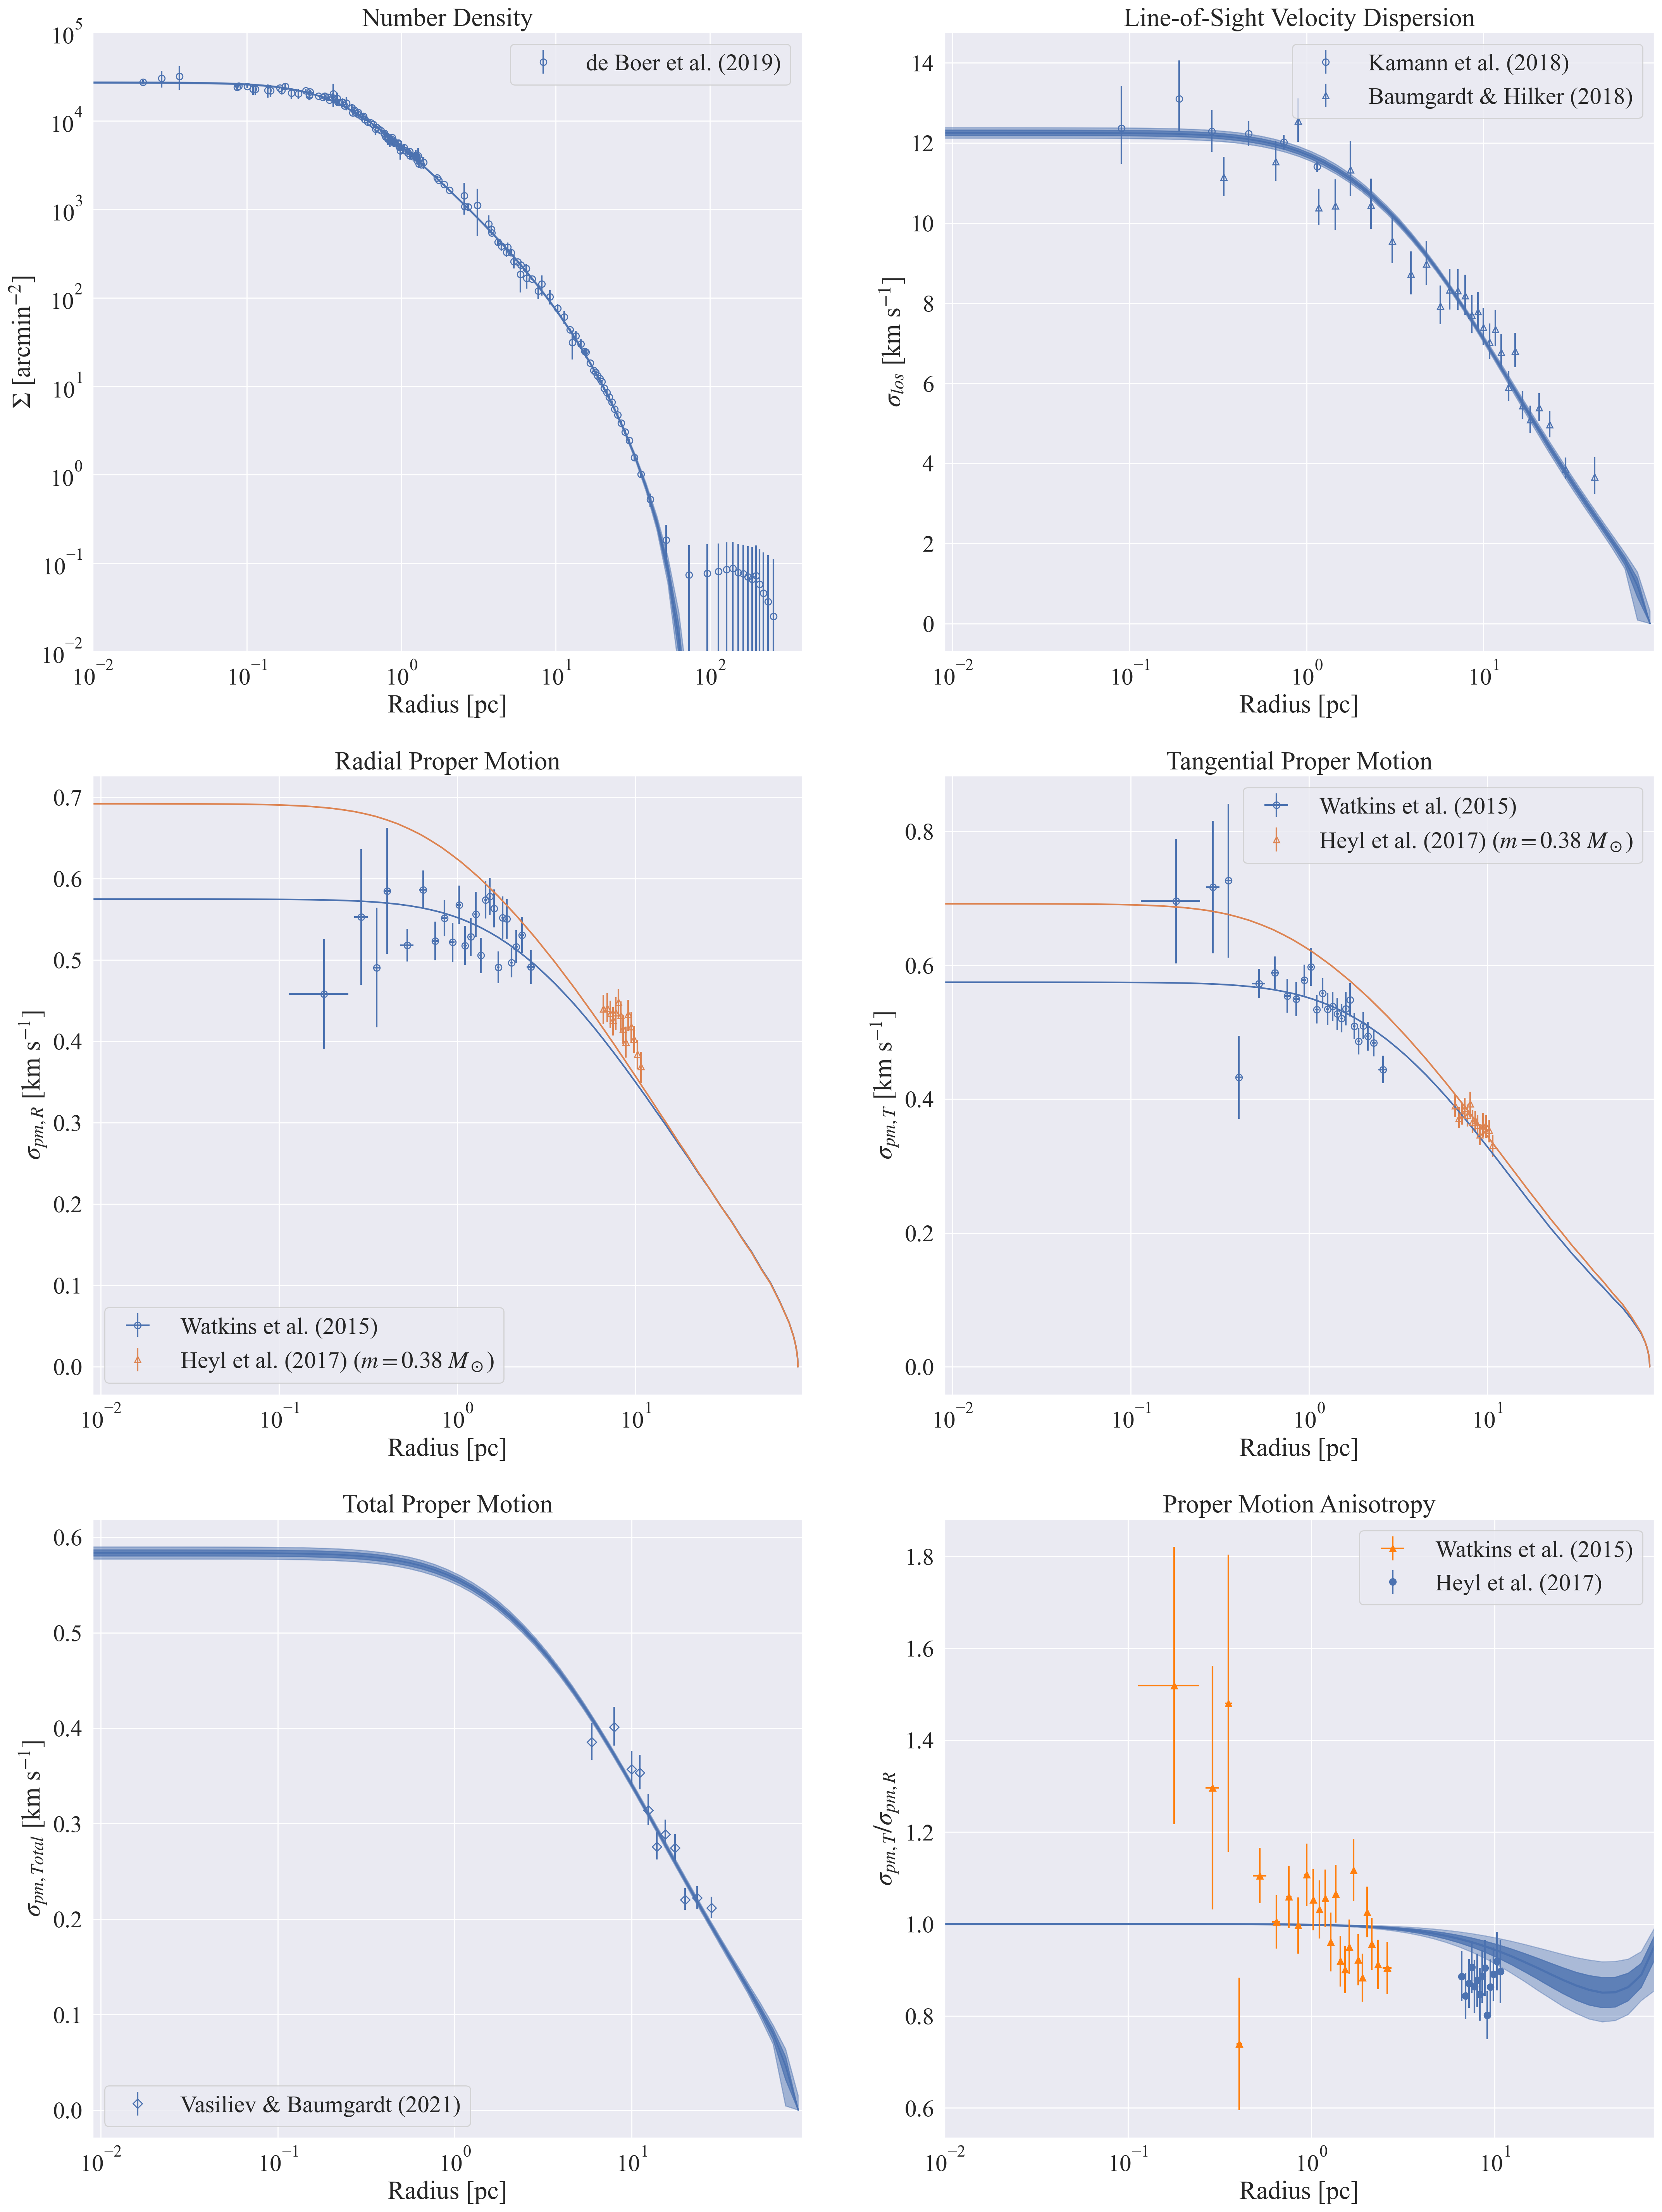
\includegraphics[width=0.8\textwidth]{figures/high_bin_model/obs_panel.png}
	\caption{Model fits to the observables for models with a $10\%$ binary fraction.}
	\label{fig:highbin_obs_panel}
\end{figure}


\begin{figure}
	\centering
	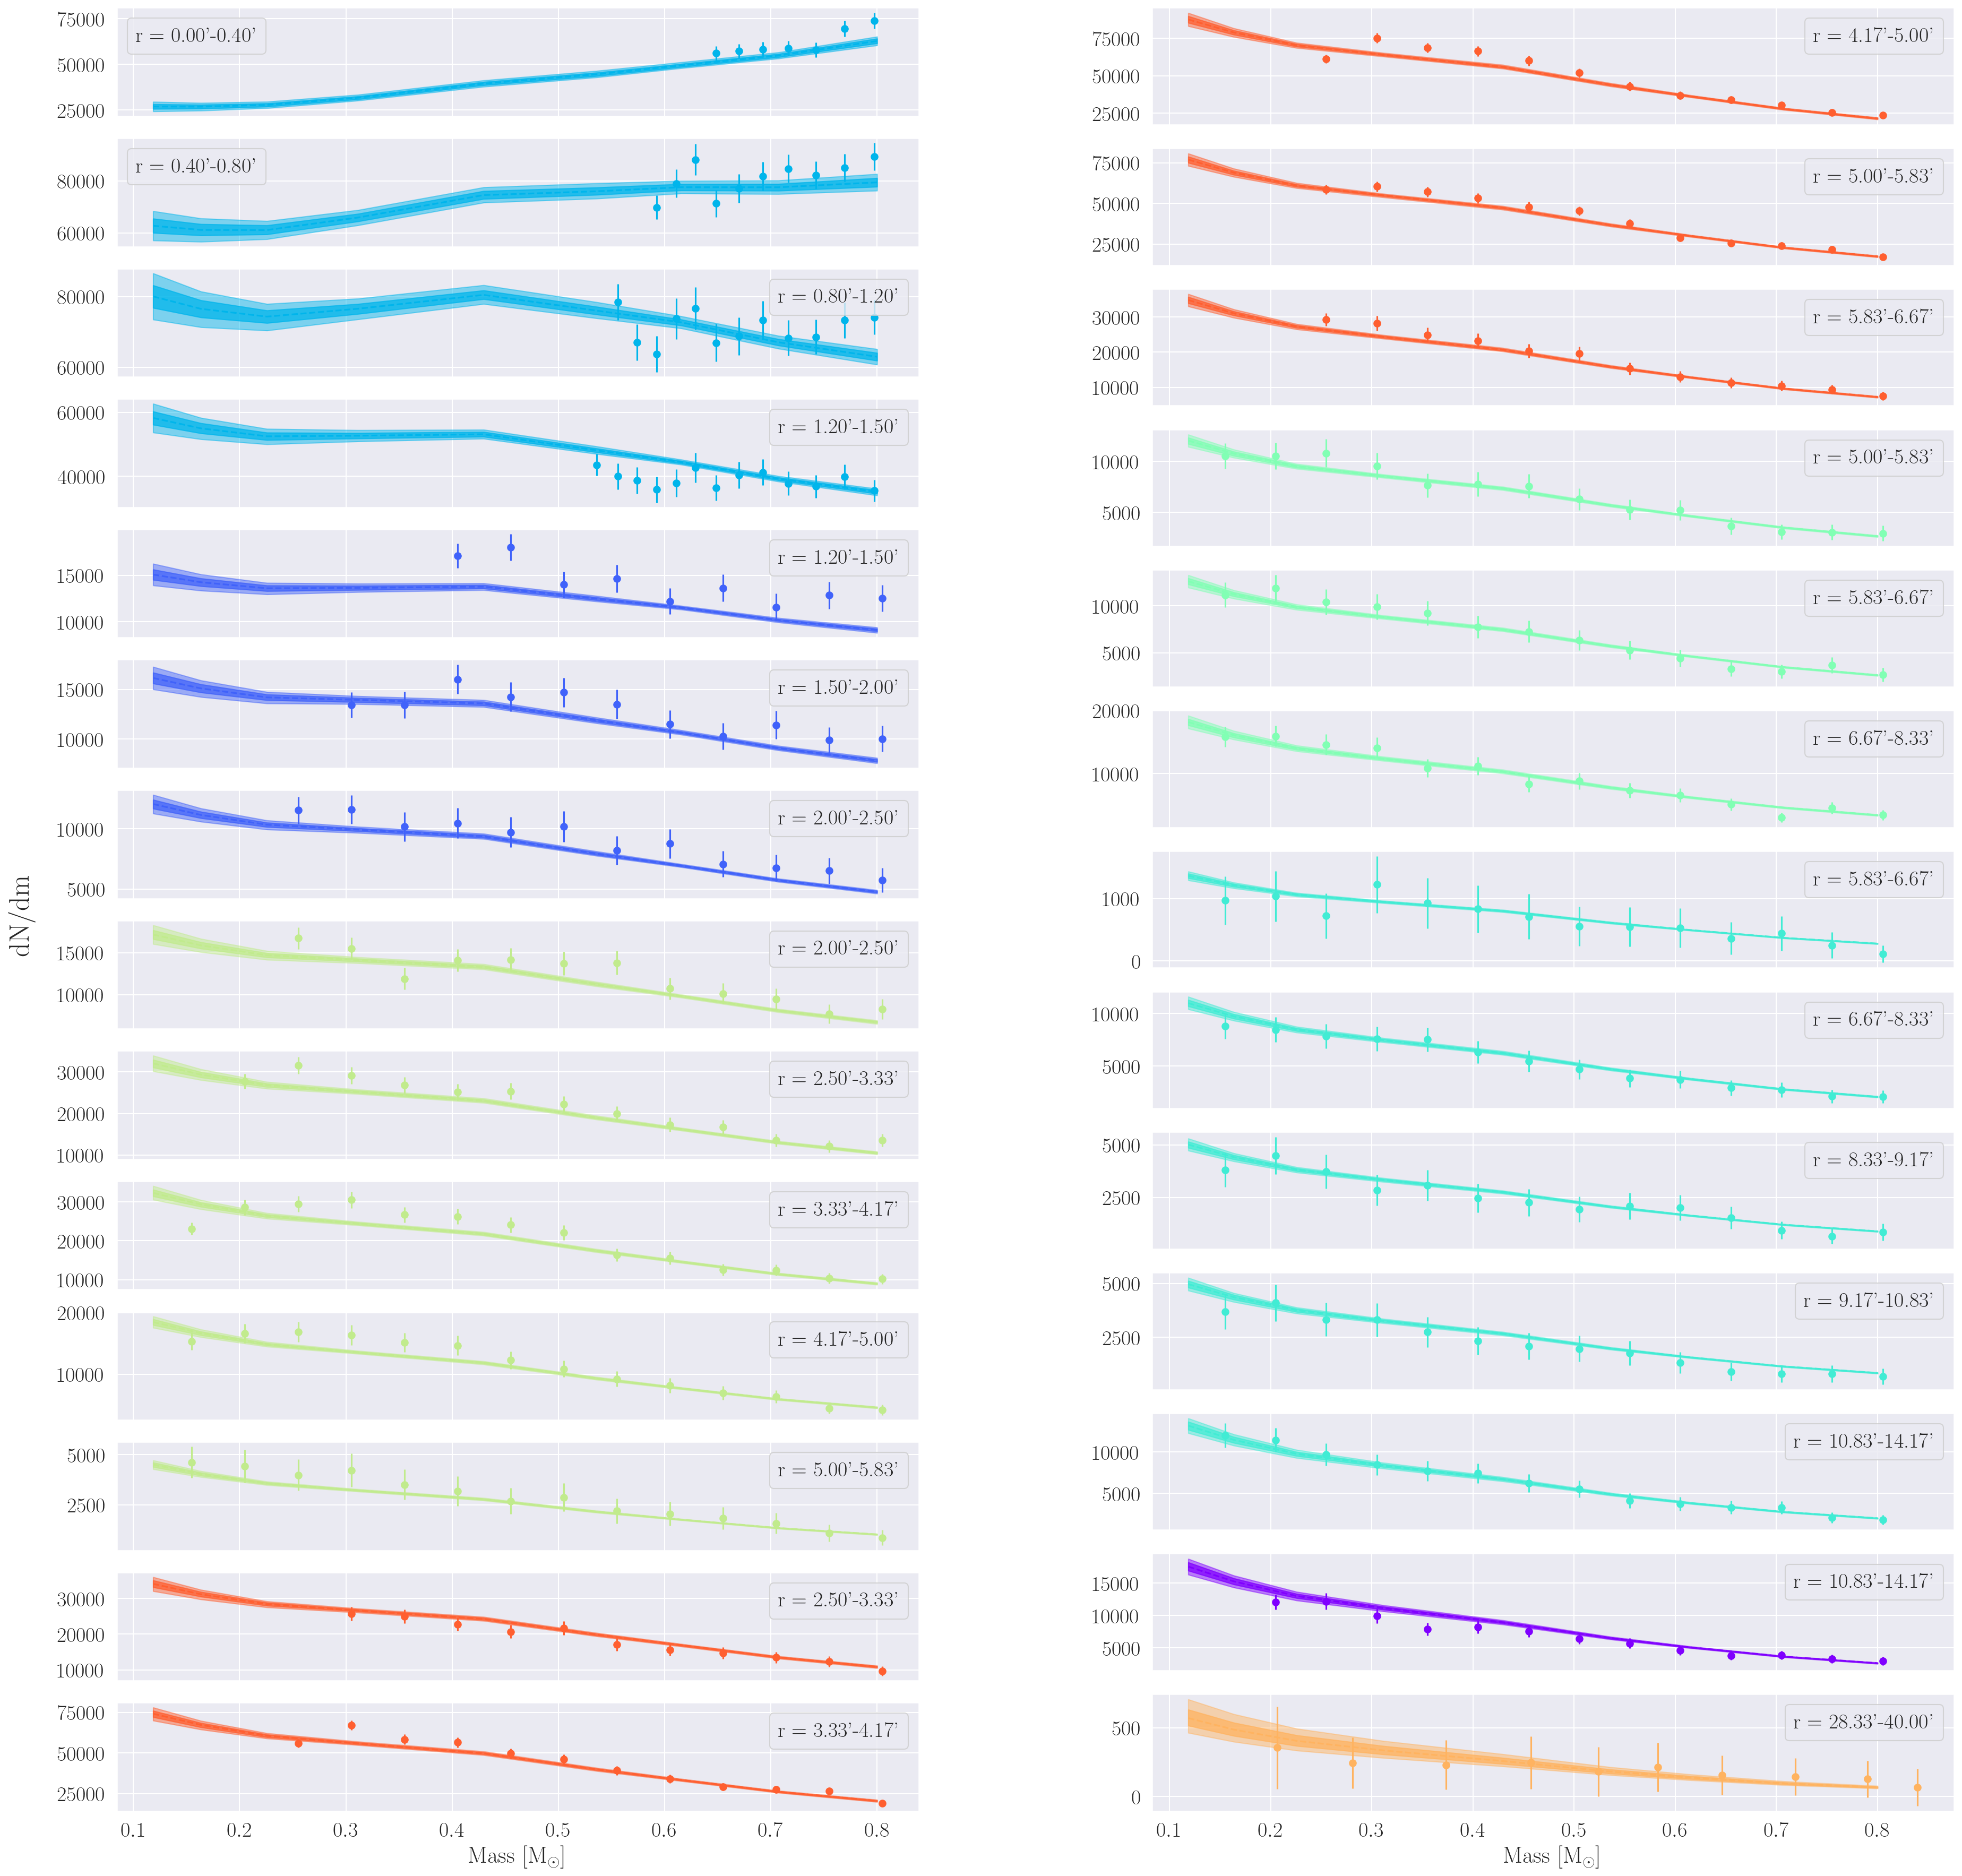
\includegraphics[width=0.8\textwidth]{figures/high_bin_model/mass_fun.png}
	\caption{Model fits to the stellar mass function data for models with a $10\%$ binary fraction.}
	\label{fig:highbin_mass_fun}
\end{figure}




